%\setcounter{chapter}{17}

 \chapter{Image Pyramids}
 \label{chapter:image_pyramids}



%In the previous chapters we have seen the power of simple linear filters to extract useful image properties. Things get a lot more interesting when many filters are used in order to represent images. In this chapter we will study some important filter ensembles. 

%We will focus on the following properties:
%\begin{itemize}
%\item Multiscale image analysis
%\item Reconstruction property
%\item Non-aliased representations
%\end{itemize}
%

% Basic references:
% http://users.utcluj.ro/~tmarita/HCI/C7-8-extra/Pyramids/RCA84.pdf

%Which properties should a filter set have?

\section{Introduction}

In \chap{\ref{chapter:linear_image_filtering}} we motivated translation invariant linear filters as a way of accounting for the fact that objects in images might appear at any location. Therefore, a reasonable way of processing an image is by manipulating pixel neighborhoods  in the same way independently on the image location. In addition to translation invariance, scale invariance is another fundamental property of images. Due to perspective projection, objects at different distances will appear with different sizes as shown in \fig{\ref{fig:birds_multiscale}}. Therefore, if we want to locate all the bird instances in this image, we will have to apply an operator that is invariant in translation and in scale. Image pyramids provide an efficient representation for space-scale invariant processing.


\begin{figure}[h!]
\centerline{
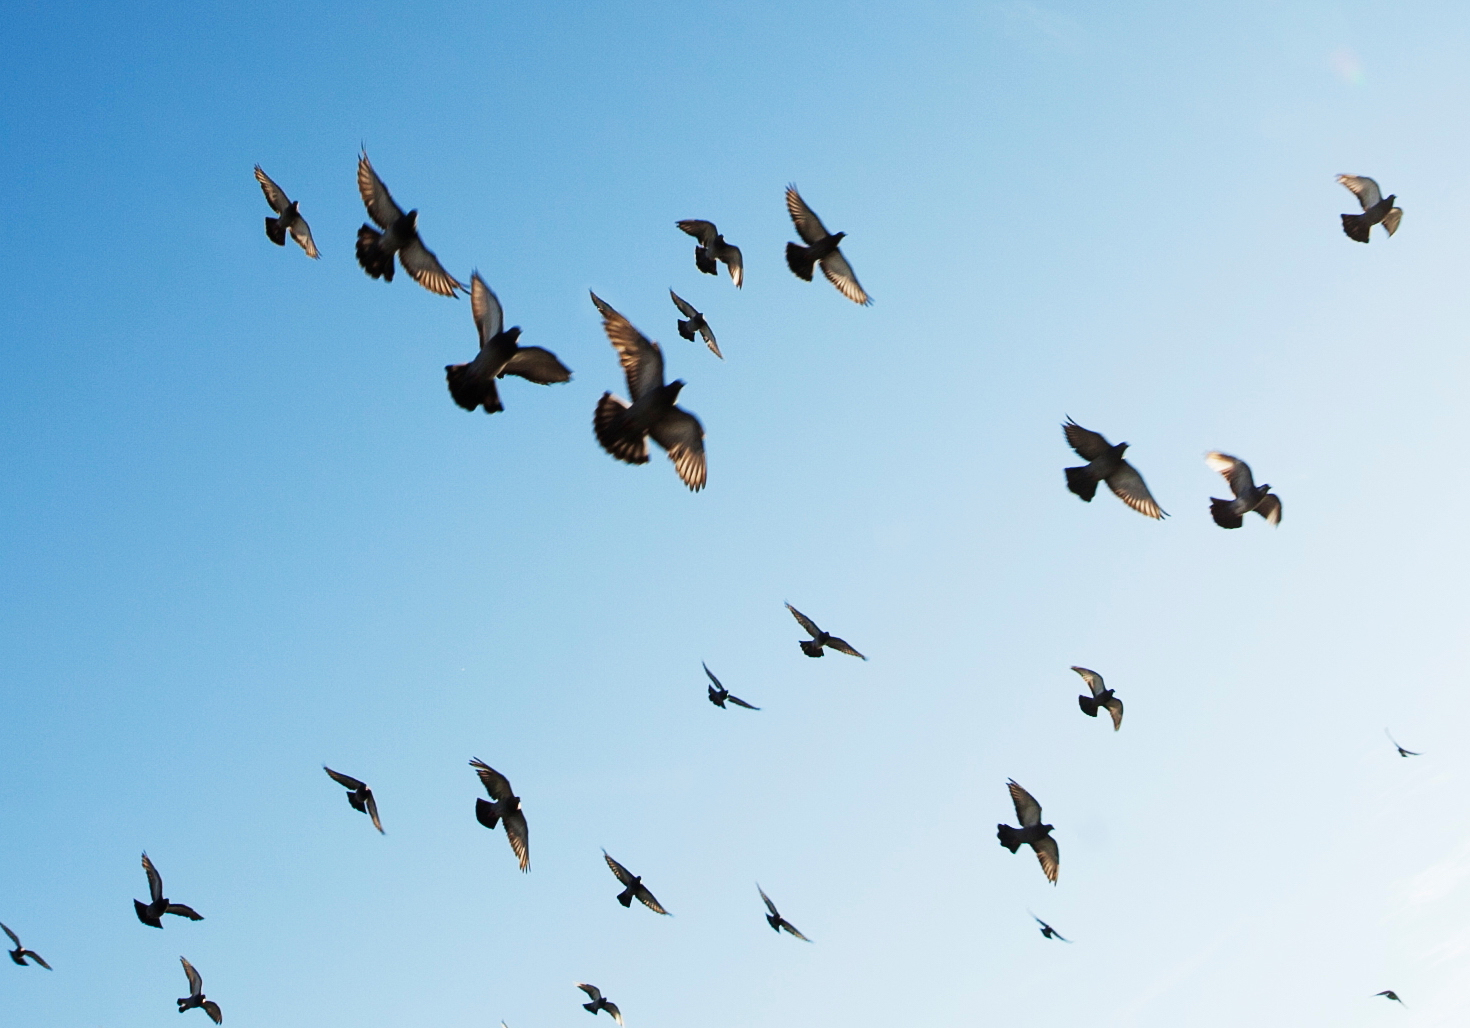
\includegraphics[width=.8\linewidth]{figures/pyramids/birds_multiscale.jpg}
}
\caption{Objects in images appear at arbitrary locations and with arbitrary image sizes.% (Image source: Antonio Torralba?).
}
\label{fig:birds_multiscale}
\end{figure}



\section{Image Pyramids and Multiscale Image Analysis}

Image information occurs over many different spatial scales.
Image pyramids (i.e., multiresolution representations for images) 
are a
useful data structure for analyzing and manipulating images over a
range of spatial scales.  Here we'll discuss three different ones, in a
progression of complexity. The first is a Gaussian pyramid, which creates versions of the input
image at multiple resolutions.  This is useful for analysis across
different spatial scales, but doesn't separate the image into
different frequency bands.  The Laplacian pyramid provides that extra
level of analysis, breaking the image into different isotropic spatial
frequency bands.  
%The Wavelet or QMF (quadrature mirror filter)
%pyramid provides some splitting of the spatial frequency bands
%according to orientation (although in a somewhat limited way).  
The
steerable pyramid provides a clean separation of the image into
different scales and orientations.  There are various other
differences between these pyramids, which we'll describe below.


As a motivating example, let's assume we want to detect the birds from \fig{\ref{fig:birds_multiscale}}. 
% using the normalized correlation approach described in section XX. 
If we have a template of a bird, normalized correlation will be able to detect only the birds that have a similar image size than the template. To introduce {\bf scale invariance},
\index{Scale invariance}
one possible solution is to change the size of the template to cover a wide range of possible sizes and apply them to the image. Then, the ensemble of templates will be able to detect birds of different sizes. The disadvantage of this approach is that it will be computationally expensive as detecting large birds will require computing convolutions with big kernels, which is very slow. Another alternative is to change the image size as shown in \fig{\ref{fig:birds_multiscale_processing}}, resulting in a {\bf multiscale image pyramid}.
\index{Multiscale image pyramid}
In this example, the original image has a resolution of 848$\times$643 pixels. Each image in the pyramid is obtained by scaling down the image from the previous level by reducing the number of pixels by a factor of $25$ percent (that is, each image in the pyramid has 3/4 of the size of the precedent image)\footnote{Downsampling is discussed in detail in \chap{\ref{chap:downsampling_and_upsampling}}.}. 


\begin{figure}[t]
\centerline{
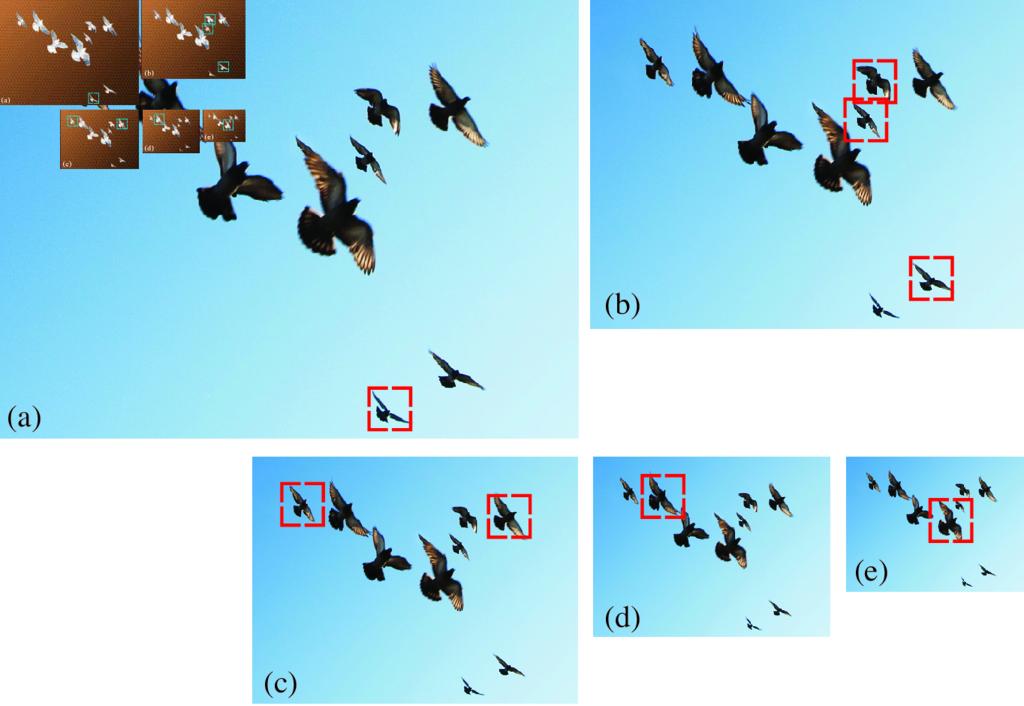
\includegraphics[width=0.8\linewidth]{figures/pyramids/multiscale_birds_boxes.eps}
}
\caption{Multiscale image pyramid. Each image is 25 percent smaller than the previous one. The red box indicates the size of a template used for detecting birds. As the size of the template is fixed; it will only be able to detect the birds that tightly fit inside the box. %Birds that are smaller or larger will not be detected.
%within a single scale. 
By running the same template across many levels in this pyramid, different instances of birds are detected at different scales.}
\label{fig:birds_multiscale_processing}
\end{figure}


Now we can use the pyramid to detect birds at different sizes using a single template. The red box in the figure denotes the size of the template used. The figure shows how birds of different sizes become detectable at, at least, one of the levels of the pyramid. This method will be more efficient as the template can be kept small and the convolutions will remain computationally efficient. 

Mutiscale image processing and image pyramids have many applications beyond scale invariant object detection. In this chapter we will describe some important image pyramids and their applications. 


\section{Linear Image Transforms}

Let's first look at some general properties of linear image transforms.  For an input image $\boldimg$ with $N$ pixels, a linear transform is:
\begin{equation}
\mathbf{r} = \mathbf{P}^\transpose \boldimg 
\end{equation}
where $\mathbf{r}$ is a vector of dimensionality $M$, and $\mathbf{P}$ is a matrix of size $N \times M$. The columns of $\mathbf{P} = \left[\mathbf{P}_0,  \mathbf{P}_1, ...,\mathbf{P}_{M-1}\right]$ are the projection vectors. The vector $\mathbf{r}$ contains the transform coefficients: $\mathbf{r}_i = \mathbf{P}_i^\transpose \boldimg$.  The vector $\mathbf{r}$ corresponds to a different representation of the image $\boldimg$ than the original pixel space. 


We are interested in transforms that are invertible, 
\index{Invertible transform}
so that we can recover the input $\boldimg$ from the projection coefficients $\mathbf{r}$:
\begin{equation}
\boldimg = \mathbf{Q} \mathbf{r} = \sum_{i=0}^{M-1} \mathbf{r}_i \mathbf{Q}_i 
\end{equation}
The columns of $\mathbf{Q}= \left[\mathbf{Q}_0,  \mathbf{Q}_1, ...,\mathbf{Q}_{M-1}\right]$ are the basis vectors. The input signal $\boldimg$ can be reconstructed as a linear combination of the basis vectors $\mathbf{Q}_i$ weighted by the representation coefficients $\mathbf{r}_i$.  

The transform $\mathbf{P}$ is said to be {\bf critically sampled} when $M=N$.  The transform is {\bf oversampled} when $M > N$, and {\bf undersampled} when $M < N$. 
The transform $\mathbf{P}$ is complete, that is, encoding all image structure, if it is invertible. If critically sampled (i.e., $M=N$) and the transform is complete, then $\mathbf{Q} = (\mathbf{P}^\transpose)^{-1}$.  If it is overcomplete (oversampled and complete), then the inverse can be obtained using the pseudoinverse $\mathbf{Q}=(\mathbf{P} \mathbf{P}^\transpose)^{-1}\mathbf{P}$.

An important special case is when the transform is {\bf self-inverting},
\index{Self-inverting transform}
then $\mathbf{P} \mathbf{P}^{\transpose} = \mathbf{I}$. The values of $\mathbf{P}$ can be real or complex (like in the Fourier transform). For complex transforms, we should replace the $\mathbf{P}^\transpose$ by $\mathbf{P}^{*\transpose}$ (i.e., complex conjugate transpose).

\marginnote{The quadrature mirror filter (QMF) transform is an example of self-inverting transform \cite{Adelson87b}. For 1D signals of length 4, the QMF transform can be written as:
\begin{equation*}
\mathbf{P}=\frac{1}{\sqrt{2}}
 \begin{bmatrix}
  1 ~& 1 ~& 0 ~& 0 \\
  1 ~& -1 ~& 0 ~& 0 \\
  0 ~& 0 ~& 1 ~& 1 \\
  0 ~& 0 ~& 1 ~& -1  
 \end{bmatrix}
\end{equation*}
This is equivalent to the convolution of the input signal with two orthogonal kernels, $[1,1]$ and $[1,-1]$, with a stride of 2.
\\[6pt]
This transform also has a multiscale version that is also self-inverting:
\begin{equation*}
\mathbf{P}=
 \begin{bmatrix}
  \frac{1}{\sqrt{2}} & -\frac{1}{\sqrt{2}} & 0 & 0 \\[5pt]
  0 & 0 & \frac{1}{\sqrt{2}} & -\frac{1}{\sqrt{2}} \\[5pt]
  \frac{1}{2} & \frac{1}{2} & \frac{1}{2} & \frac{1}{2} \\[5pt] 
  \frac{1}{2} & \frac{1}{2} & -\frac{1}{2} & -\frac{1}{2} 
 \end{bmatrix}
\end{equation*}
You can check that in both cases $\mathbf{Q} = \left( \mathbf{P^\transpose} \right) ^{-1} = \mathbf{P^\transpose}$.
These transforms can be extended to 2D. 
}


\section{Gaussian Pyramid}


%
%
%
%\begin{figure}
%\centerline{
%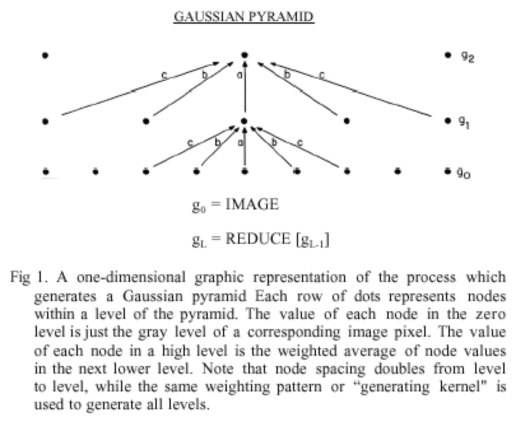
\includegraphics[width=0.7\linewidth]{figures/pyramids/gausspyr.jpg}
%}
%\caption{Computation for the Gaussian pyramid.}
%\label{fig:gausspyr}
%\end{figure}
%
%
%\begin{figure}
%\centerline{
%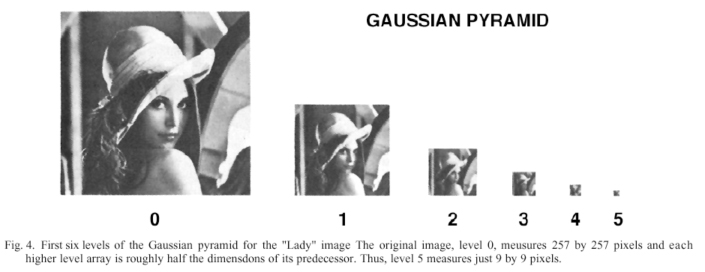
\includegraphics[width=0.8\linewidth]{figures/pyramids/gpyr.jpg}
%}
%\caption{Gaussian pyramid example}
%\label{fig:gpyr}
%\end{figure}
%
%
%\begin{figure}
%\centerline{
%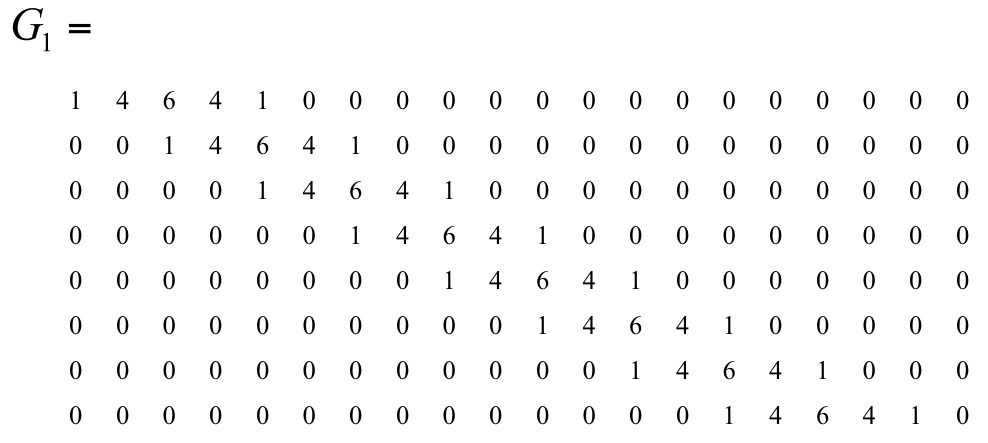
\includegraphics[width=0.8\linewidth]{figures/pyramids/gpnums1.jpg}
%}
%\centerline{
%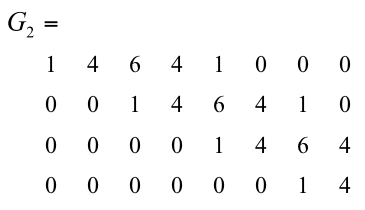
\includegraphics[width=0.4\linewidth]{figures/pyramids/gpnums2.jpg}
%}
%\centerline{
%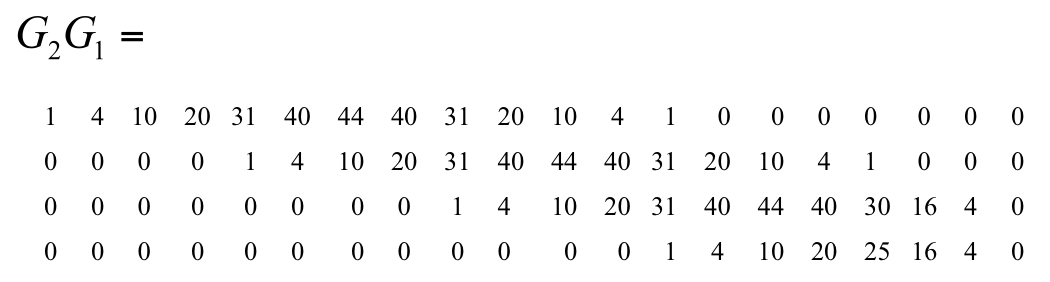
\includegraphics[width=0.8\linewidth]{figures/pyramids/gpnums3.jpg}
%}
%\caption{Gaussian pyramid matrix numbers}
%\label{fig:gpnums}
%\end{figure}


We'd like to make a recursive algorithm for creating a multiresolution version of an image.  
\index{Multiresolution}
A Gaussian filter is a natural
one to use to blur out an image, since the multiple successive application of a Gaussian filter is equivalent to application of a single, wider
Gaussian filter.

Here's an elegant, efficient algorithm for making a resolution--reduced version of an input image.  It involves two steps:  convolving the
image with a low-pass filter (e.g., using the fourth binomial filter $\mathbf{b}_4 = [1, 4, 6, 4, 1]$ / 16, normalized to sum to 1, separably in each dimension), and then subsampling by a factor of 2 the result. Each level is obtained by filtering the previous level with the fourth binomial filter with a stride of 2 (on each dimension). Applied recursively, this algorithm generates a sequence of images,  subsequent ones being smaller, lower resolution versions of the earlier ones in the processing.
% Drawing the blocks of first level:


\Fig{\ref{fig:gausspyr}} shows the Gaussian pyramid of an image with six levels. Each level has half the resolution of the previous level.  

\begin{figure}[t]
\centerline{
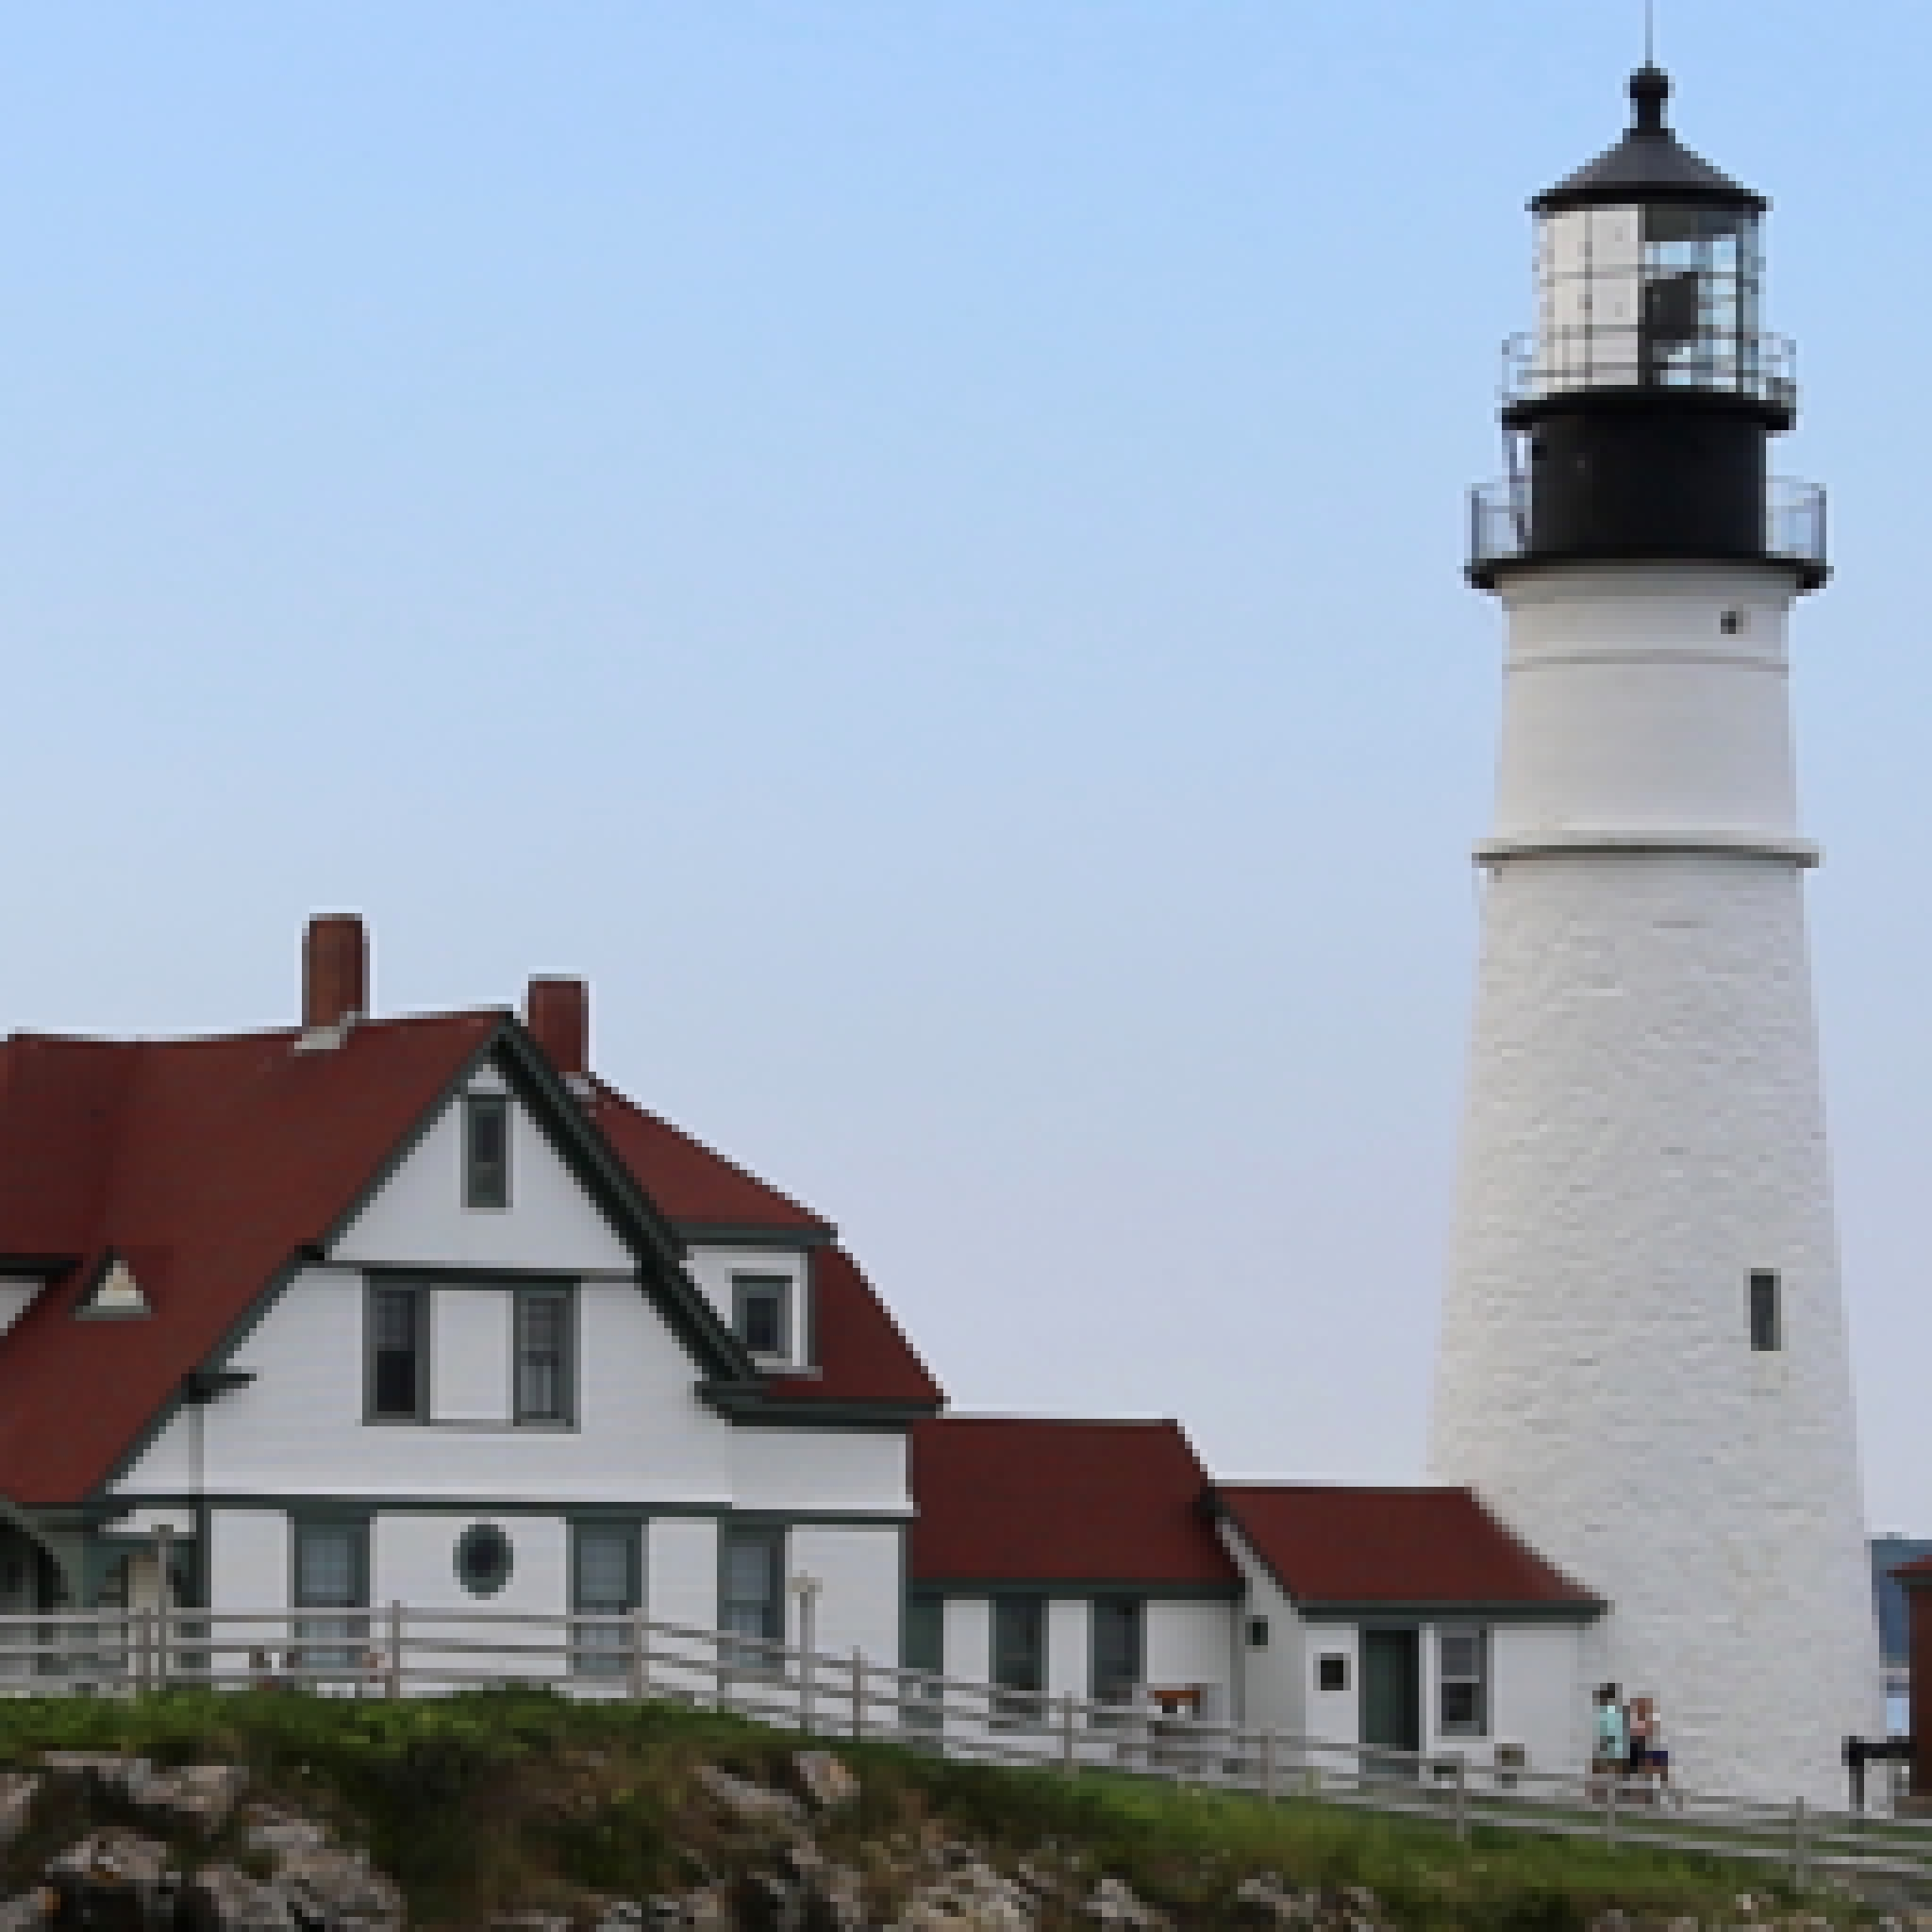
\includegraphics[width=0.5\linewidth]{figures/pyramids/gaussianPyr_1.jpg}
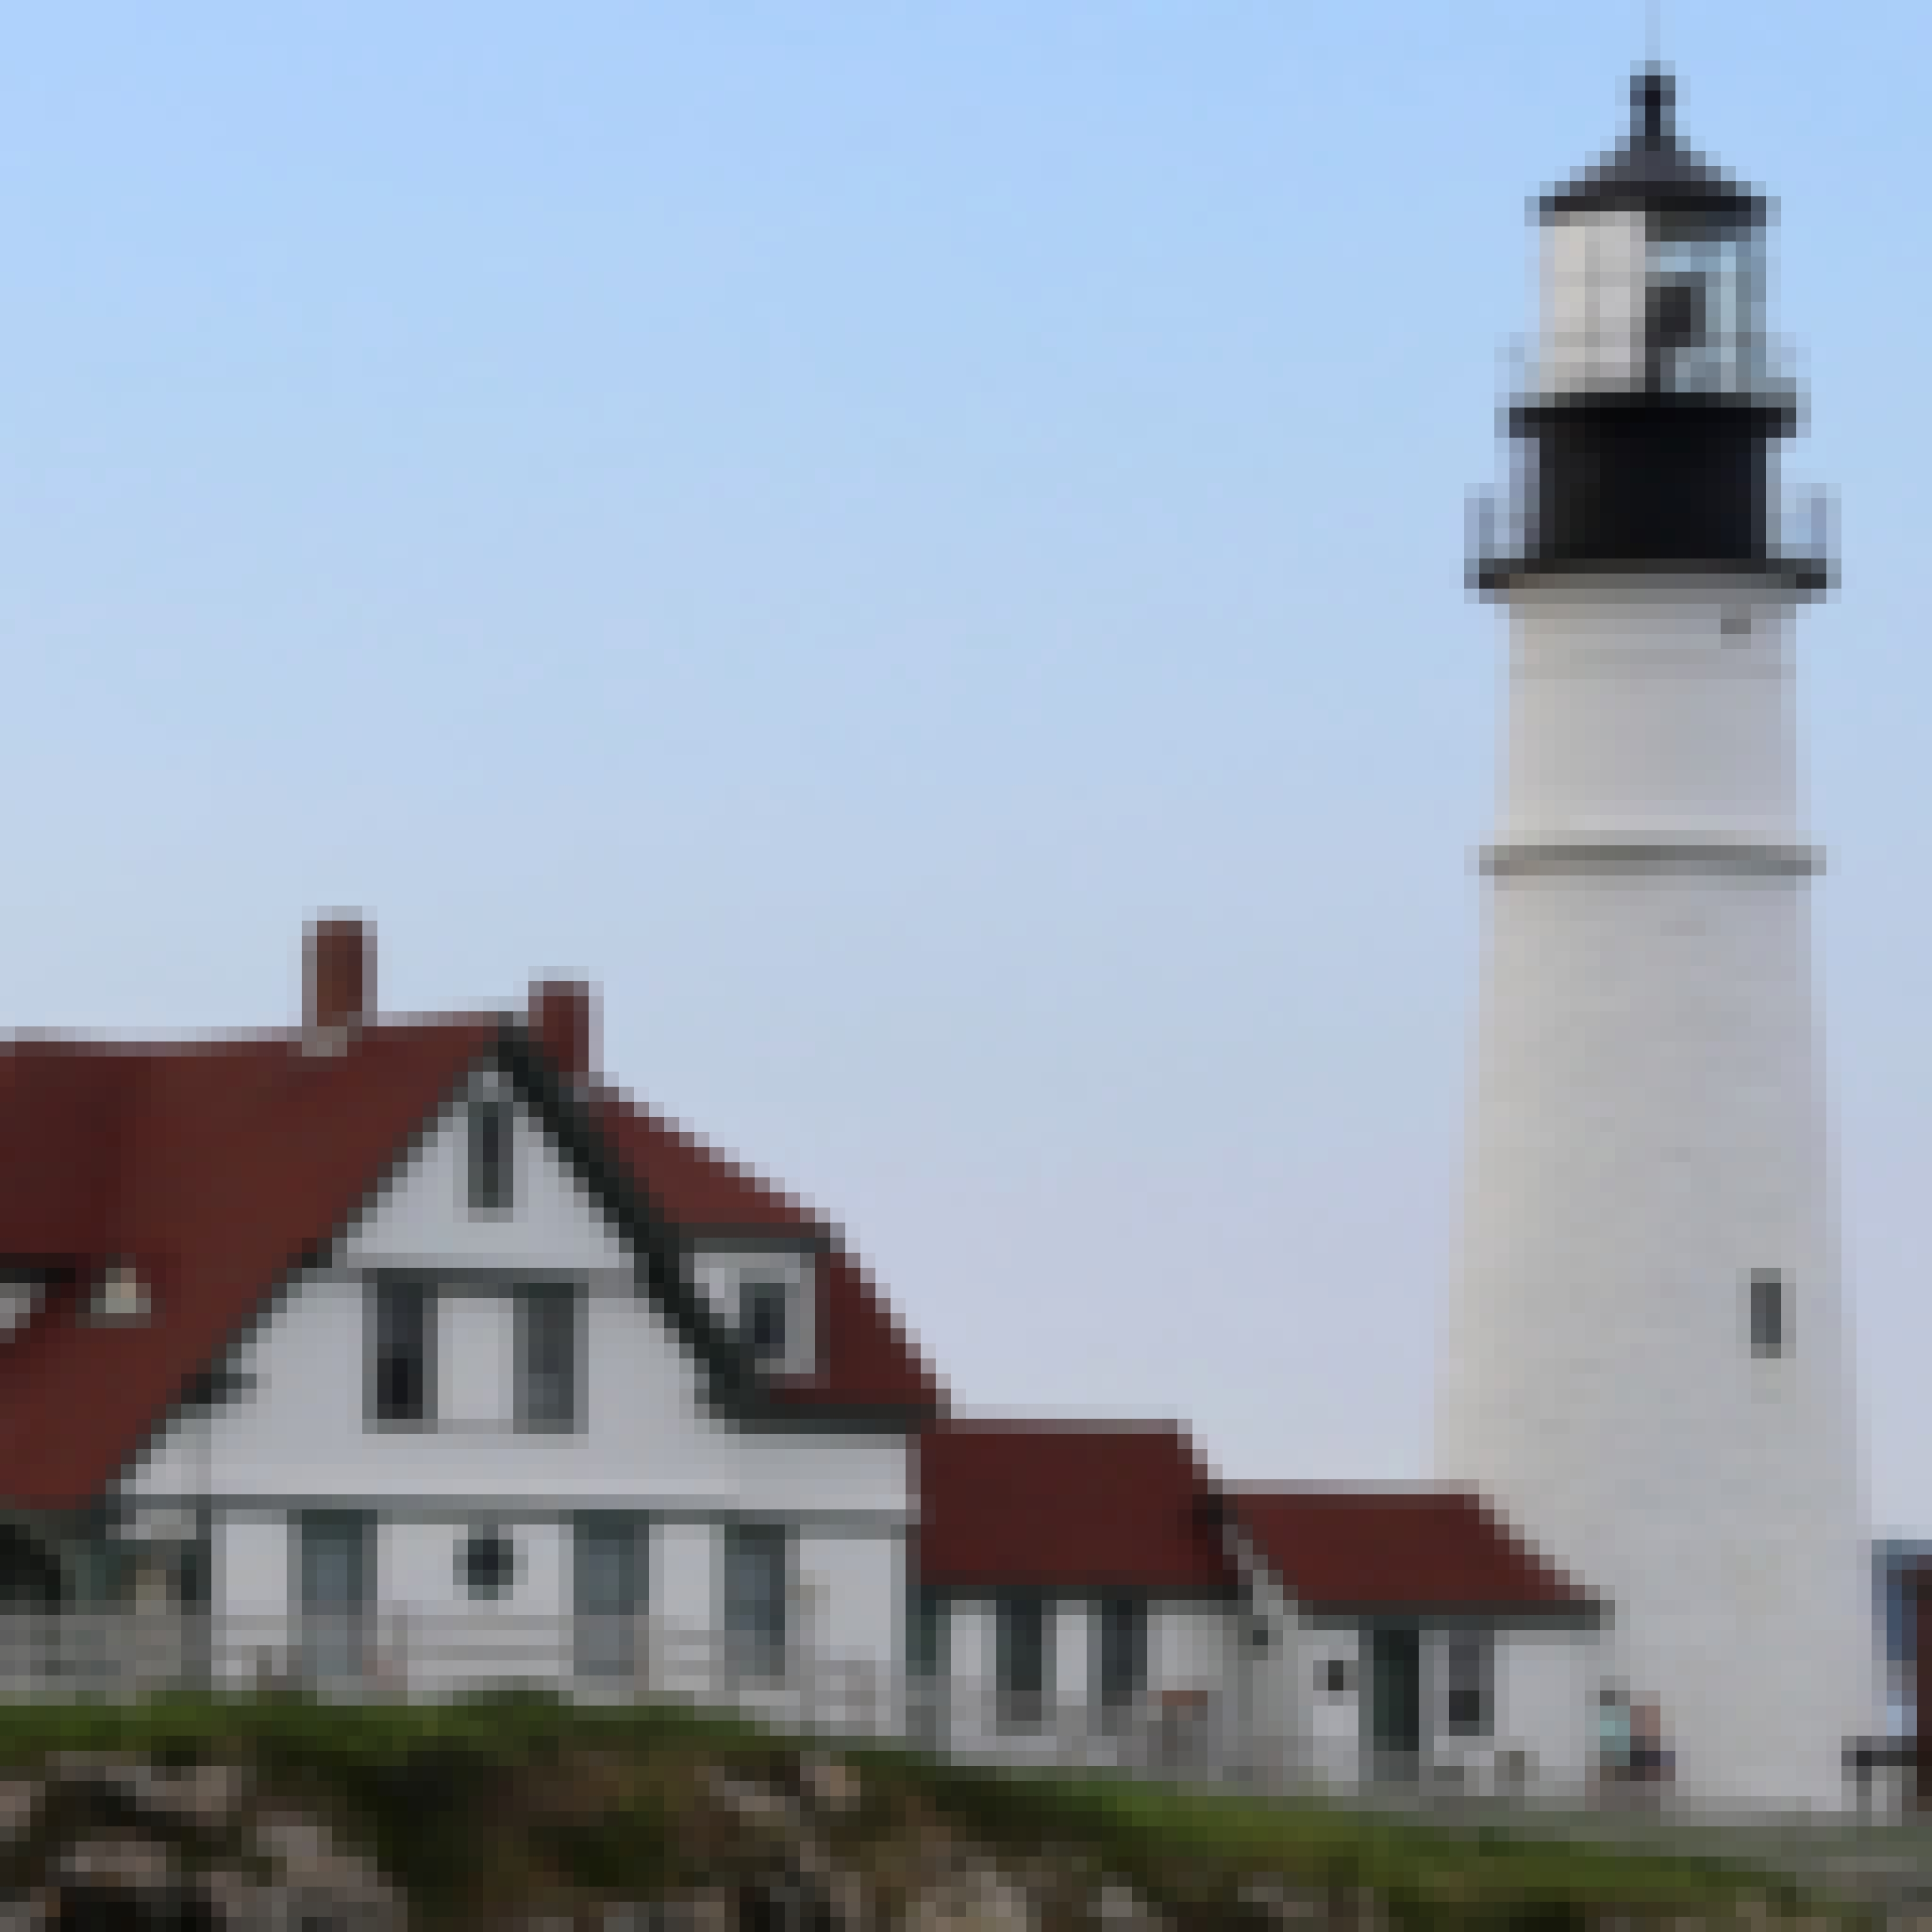
\includegraphics[width=0.25\linewidth]{figures/pyramids/gaussianPyr_2.jpg}

\includegraphics[width=0.125\linewidth]{figures/pyramids/gaussianPyr_3.jpg}
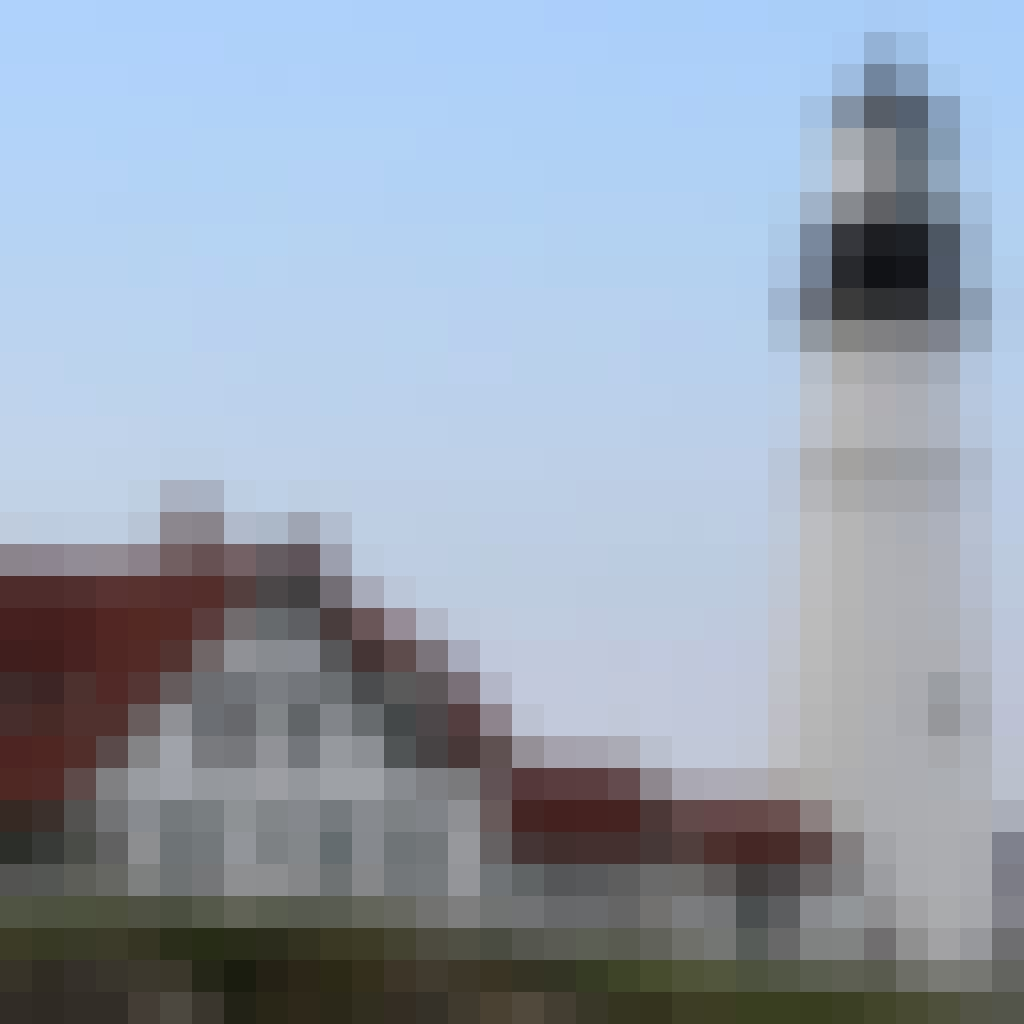
\includegraphics[width=0.0625\linewidth]{figures/pyramids/gaussianPyr_4.jpg}
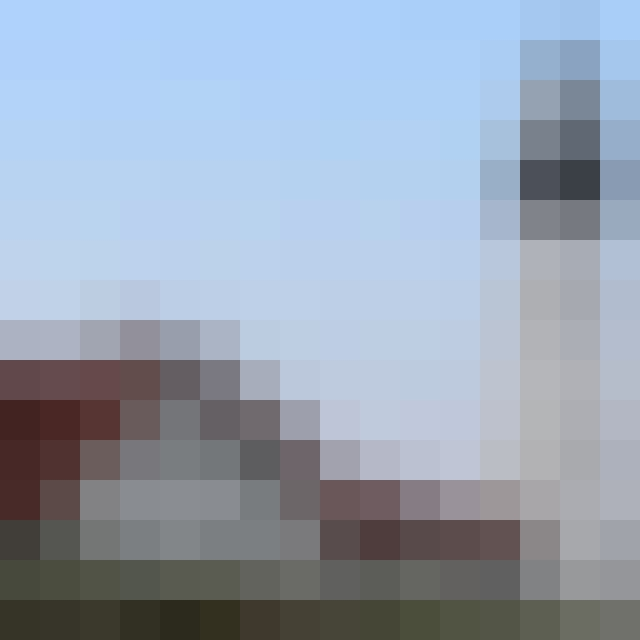
\includegraphics[width=0.03125\linewidth]{figures/pyramids/gaussianPyr_5.jpg}

\includegraphics[width=0.015625\linewidth]{figures/pyramids/gaussianPyr_6.jpg}
}
\caption{Gaussian pyramid with six levels. The first level, $\mathbf{g}_0$, is the input image. The Gaussian pyramid is built for each color channel independently.}
\label{fig:gausspyr}
\end{figure}



To make the filters more intuitive, it is useful to write the two steps in matrix form. 
The following matrix shows the recursive construction of  level $k+1$ of the Gaussian pyramid for a one-dimensional (1D) image:
\begin{equation}
\mathbf{g}_{k+1} = \mathbf{D}_k \mathbf{B}_k \mathbf{g}_k = \mathbf{G}_k \mathbf{g}_k
\end{equation}
where $\mathbf{D}_k$ is the downsampling operator, $\mathbf{B}_k$ is the convolution with the fourth binomial filter, and $\mathbf{G}_k = \mathbf{D}_k \mathbf{B}_k$ is the blur-and-downsample operator for level $k$.


\marginnote{One {\bf block} of the Gaussian pyramid computation.
\\[6pt]
\centerline{
\tikzset{
  block/.style    = {draw, thin, rectangle, minimum height = 1.5em,  minimum width = 1.5em},
  sum/.style      = {draw, circle, minimum size=.4cm}, % Adder
  input/.style    = {coordinate}, % Input
  output/.style   = {coordinate}, % Output
  x/.style   = {coordinate} % Output
}
\begin{tikzpicture}[auto, thin, node distance=1.2cm, >=latex]%triangle 45]
\draw
	node [input] (x0) {}
	node [right of=x0, node distance=0cm] (x0p) {$\mathbf{g}_k$}
	%node [input] (x0p) {$x_0$}
	node [block, right of=x0p] (g0) {$\mathbf{G}_k$}
	node [right of=g0] (x1) {$\mathbf{g}_{k+1}$};
       % Joining blocks. 
	%\draw[-](x0) -- node {} (x0p);
	\draw[->](x0p) -- node {} (g0);
	\draw[->](g0) -- node {} (x1);
	%\draw [->] (a3) -| node[pos=0.99, right] {{\tiny $-$}} (sum);
\end{tikzpicture}
}
}

We call the  sequence of images  $\mathbf{g}_0,  \mathbf{g}_1, . . ., \mathbf{g}_N$  as the Gaussian pyramid.  The first level of the Gaussian pyramid is the input image: $\mathbf{g}_0=\boldimg$.


It is useful to check a concrete example. If $\mathbf{x}$ is a 1D signal of length 8, and if we assume zero boundary conditions, the matrices for computing $\mathbf{g}_1$ are:
\begin{equation}
\mathbf{G}_0 = \mathbf{D}_0 \mathbf{B}_0 =
\begin{bmatrix}
  1 ~& 0 ~& 0 ~& 0 ~& 0 ~& 0 ~& 0 ~& 0 \\
  0 ~& 0 ~& 1 ~& 0 ~& 0 ~& 0 ~& 0 ~& 0 \\
  0 ~& 0 ~& 0 ~& 0 ~& 1 ~& 0 ~& 0 ~& 0 \\
  0 ~& 0 ~& 0 ~& 0 ~& 0 ~& 0 ~& 1 ~& 0
 \end{bmatrix}
 \frac{1}{16}
 \begin{bmatrix}
  6 ~& 4 ~& 1 ~& 0 ~& 0 ~& 0 ~& 0 ~& 0 \\
  4 ~& 6 ~& 4 ~& 1 ~& 0 ~& 0 ~& 0 ~& 0 \\
  1 ~& 4 ~& 6 ~& 4 ~& 1 ~& 0 ~& 0 ~& 0 \\
  0 ~& 1 ~& 4 ~& 6 ~& 4 ~& 1 ~& 0 ~& 0 \\
  0 ~& 0 ~& 1 ~& 4 ~& 6 ~& 4 ~& 1 ~& 0 \\
  0 ~& 0 ~& 0 ~& 1 ~& 4 ~& 6 ~& 4 ~& 1 \\
  0 ~& 0 ~& 0 ~& 0 ~& 1 ~& 4 ~& 6 ~& 4 \\
  0 ~& 0 ~& 0 ~& 0 ~& 0 ~& 1 ~& 4 ~& 6 
\end{bmatrix}
\end{equation}
Multiplying the two matrices:
\begin{equation}
\mathbf{g}_{1} = \mathbf{G}_0 \boldimg = 
 \frac{1}{16}
 \begin{bmatrix}
  6 ~& 4 ~& 1 ~& 0 ~& 0 ~& 0 ~& 0 ~& 0 \\
  1 ~& 4 ~& 6 ~& 4 ~& 1 ~& 0 ~& 0 ~& 0 \\
  0 ~& 0 ~& 1 ~& 4 ~& 6 ~& 4 ~& 1 ~& 0 \\
  0 ~& 0 ~& 0 ~& 0 ~& 1 ~& 4 ~& 6 ~& 4 
 \end{bmatrix}
 \boldimg
 \end{equation}
the first level of the Gaussian pyramid is a signal $\mathbf{g}_1$ with length 4. Applying the recursion we can write the output of each level as a function of the input $\boldimg$:  $\mathbf{g}_{2} = \mathbf{G}_1 \mathbf{G}_0 \boldimg$, $\mathbf{g}_{3} = \mathbf{G}_2 \mathbf{G}_1 \mathbf{G}_0 \boldimg$, and so on. 
 


%
%
%Fig.~\ref{fig:gpnums} shows a matrix which shows the contributions of each
%pixel of a (1-d) image in the Gaussian pyramid image two levels above
%it in the pyramid.  Note the large spatial extent of the low-pass
%filtering, but accomplished much more efficiently than a naive
%filtering with the equivalent low-pass filter all in one step.
%
%The Gaussian pyramid is useful for coarse-to-fine processing of
%images--using analysis at a coarse resolution to initialize processing
%at a finer level of detail.  This is shown in Fig.~\ref{fig:gpyr}.

%
%\begin{figure}
%\centerline{
%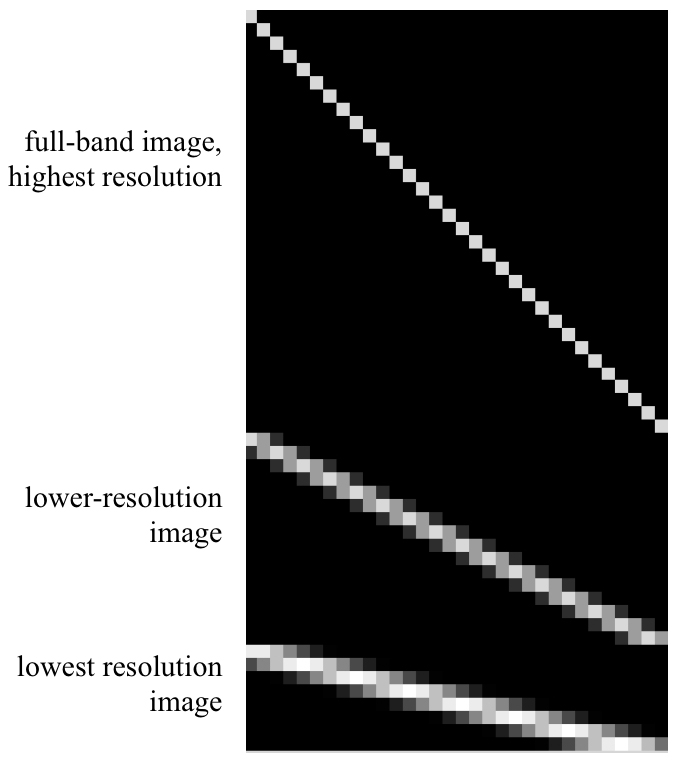
\includegraphics[width=0.5\linewidth]{figures/pyramids/gpyrmat.jpg}
%}
%\caption{Gaussian pyramid matrix image}
%\label{fig:gpyrmat}
%\end{figure}
%
%

%Fig.~\ref{fig:gpyrmat}
%shows the equivalent matrix for a simple, 3-level Gaussian pyramid
%(the pyramid is actually constructed more efficiently than by performing
%this matrix multiplication).    This matrix generates 3 versions of
%the image:  one a full resolution, a second at half the (linear) resolution,
%and a 3rd at 1/4 the resolution of the original.

\section{Laplacian Pyramid}

In the Gaussian pyramid, each level losses some of the fine image details available in the previous level. %The goal of the Laplacian pyramid is to represent, at each level, what is present in a Gaussian pyramid image of one level, but not present at the level below it. 
The {\bf Laplacian pyramid} \cite{Burt83} is simple:  it represents, at each level, what
is present in a Gaussian pyramid image of one level, but not present
at the level below it.  We calculate that by expanding the
lower-resolution Gaussian pyramid image to the same pixel resolution
as the neighboring higher-resolution Gaussian pyramid image, then
subtracting the two.  This calculation is made in a recursive,
telescoping fashion. 




% Drawing the blocks of first level:
Let's look at the steps for calculating a Laplacian pyramid.
What we want is to compute the difference between $\mathbf{g}_k$ and $\mathbf{g}_{k+1}$. To do this first we need to upsample the image $\mathbf{g}_{k+1}$ so that it has the same size as $\mathbf{g}_k$. Let $\mathbf{F}_k = \mathbf{B}_k \mathbf{U}_k$ be the upsample-and-blur operator for pyramid level $k$.  The operator $\mathbf{F}_k$ applies first the upsampling operator $\mathbf{U}_k$, that inserts zeros between samples, followed by blurring by the same filter $\mathbf{B}_k$ than the one we used for the Gaussian pyramid. The Laplacian pyramid coefficients, $\mathbf{l}_k$, at pyramid level $k$, are:  
%% we must interpolate the image
%% back up to full size before subtracting it from the original.  The
%% upConv function does upsampling (padding with zeros between
%% samples) followed by convolution.  This can be done using the
%% lowpass filter that was applied before subsampling or it can be
%% done with a different filter.
%\begin{equation}
%L_n = (I_n - F_n G_n) x_n,
%\end{equation}
\begin{equation}
\mathbf{l}_{k} =  \mathbf{g}_k - \mathbf{F}_k \mathbf{g}_{k+1} =  (\mathbf{I}_k - \mathbf{F}_k \mathbf{G}_k) \mathbf{g}_{k} = \mathbf{L}_k \mathbf{g}_{k}
\label{eqn:laplacian_pyr_coef}
\end{equation}


\marginnote{One {\bf block} of the Laplacian pyramid computation.
\\[6pt]
\centerline{
\tikzset{
  block/.style    = {draw, thin, rectangle, minimum height = 1.5em,  minimum width = 1.5em},
  sum/.style      = {draw, circle, minimum size=.4cm}, % Adder
  input/.style    = {coordinate}, % Input
  output/.style   = {coordinate}, % Output
  x/.style   = {coordinate} % Output
}
\begin{tikzpicture}[auto, thin, node distance=1.2cm, >=latex]%triangle 45]
\draw
	node [input] (x0) {}
	node [right of=x0, node distance=0cm] (x0p) {$\mathbf{g}_k$}
	%node [input] (x0p) {$x_0$}
	node [block, right of=x0p] (g0) {$\mathbf{G}_k$}
        node [block, below of=g0] (f0) {$\mathbf{F}_k$}
	node [sum, left of=f0] (suma0) {}
	node [right of=g0] (x1) {$\mathbf{g}_{k+1}$}
	node [below of=suma0] (l0) {$\mathbf{l}_k$};
       % Joining blocks. 
	%\draw[-](x0) -- node {} (x0p);
	\draw[->](x0p) -- node {} (g0);
	\draw[->](x0p) -- node[pos=0.99, left] {{\tiny $+$}} (suma0);
	\draw[->](f0) -- node[pos=0.99, below] {{\tiny $-$}} (suma0);
	\draw[->](x1) |- node {} (f0);
	\draw[->](g0) |- node {} (x1);
	\draw[->](suma0) -- node {} (l0);
	%\draw [->] (a3) -| node[pos=0.99, right] {{\tiny $-$}} (sum);
\end{tikzpicture}
}
}[-1in]

\Fig{\ref{fig:laplacpyr}} shows the resulting Laplacian pyramid for an image. To compute a Laplacian pyramid with $N$ levels, we need to first compute the Gaussian pyramid of the input image with $N+1$ levels. The last level of this pyramid is the smallest level of the Gaussian pyramid used to compute the Laplacian pyramid and is called the low-pass residual.
\index{Low-pass residual}


\begin{figure}[t]
\centerline{
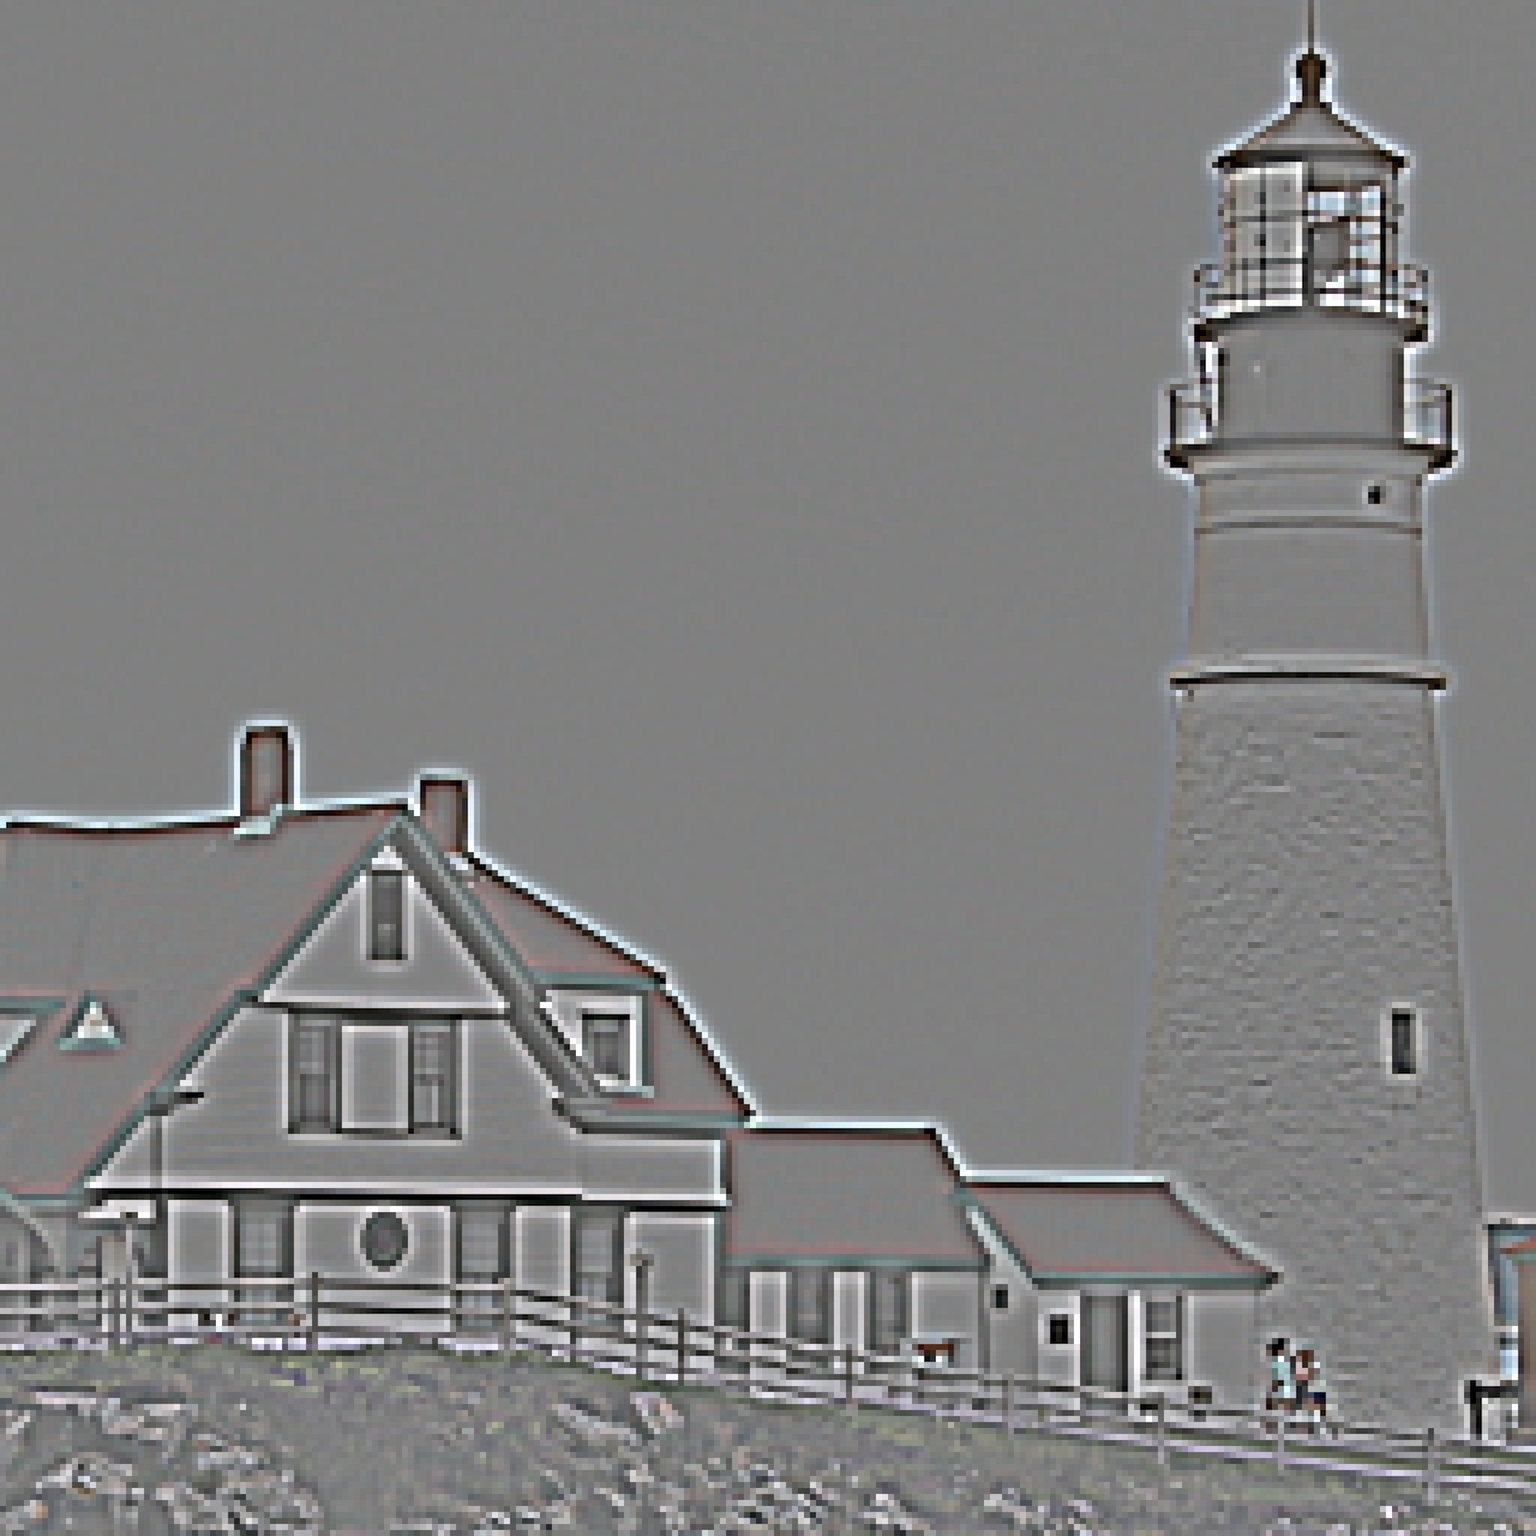
\includegraphics[width=0.48\linewidth]{figures/pyramids/laplacianPyr_1.jpg}
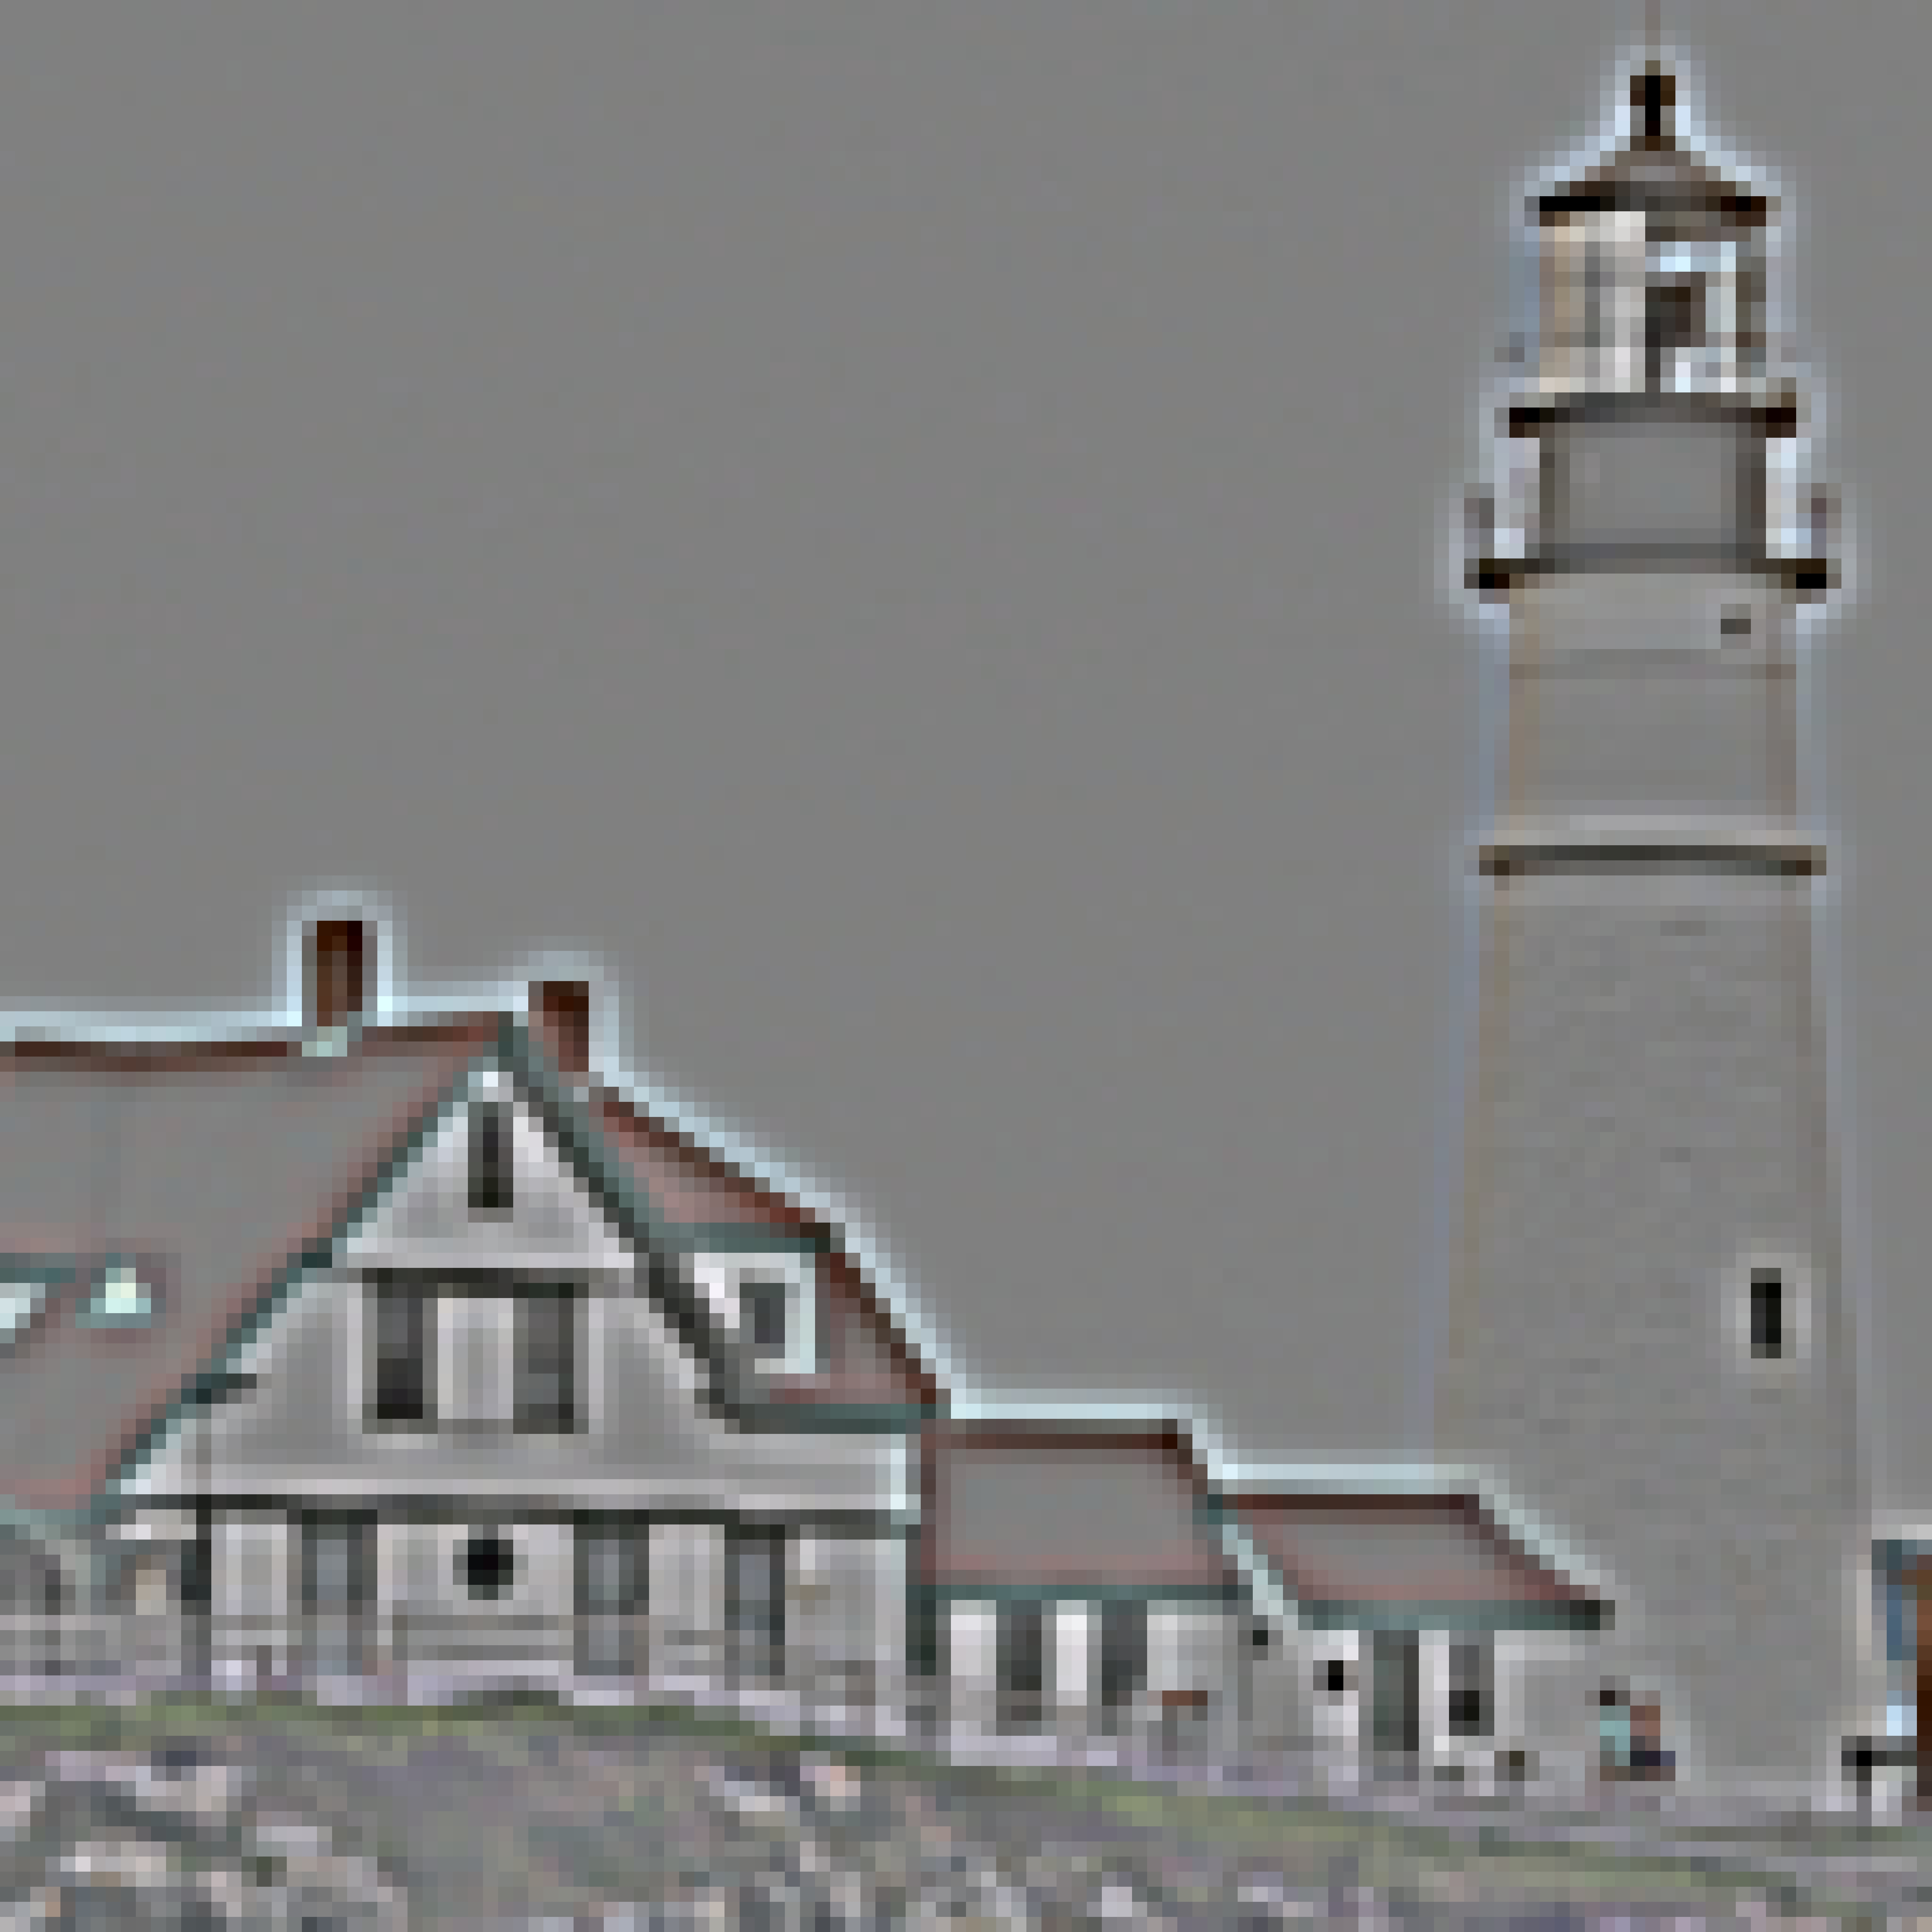
\includegraphics[width=0.24\linewidth]{figures/pyramids/laplacianPyr_2.jpg}
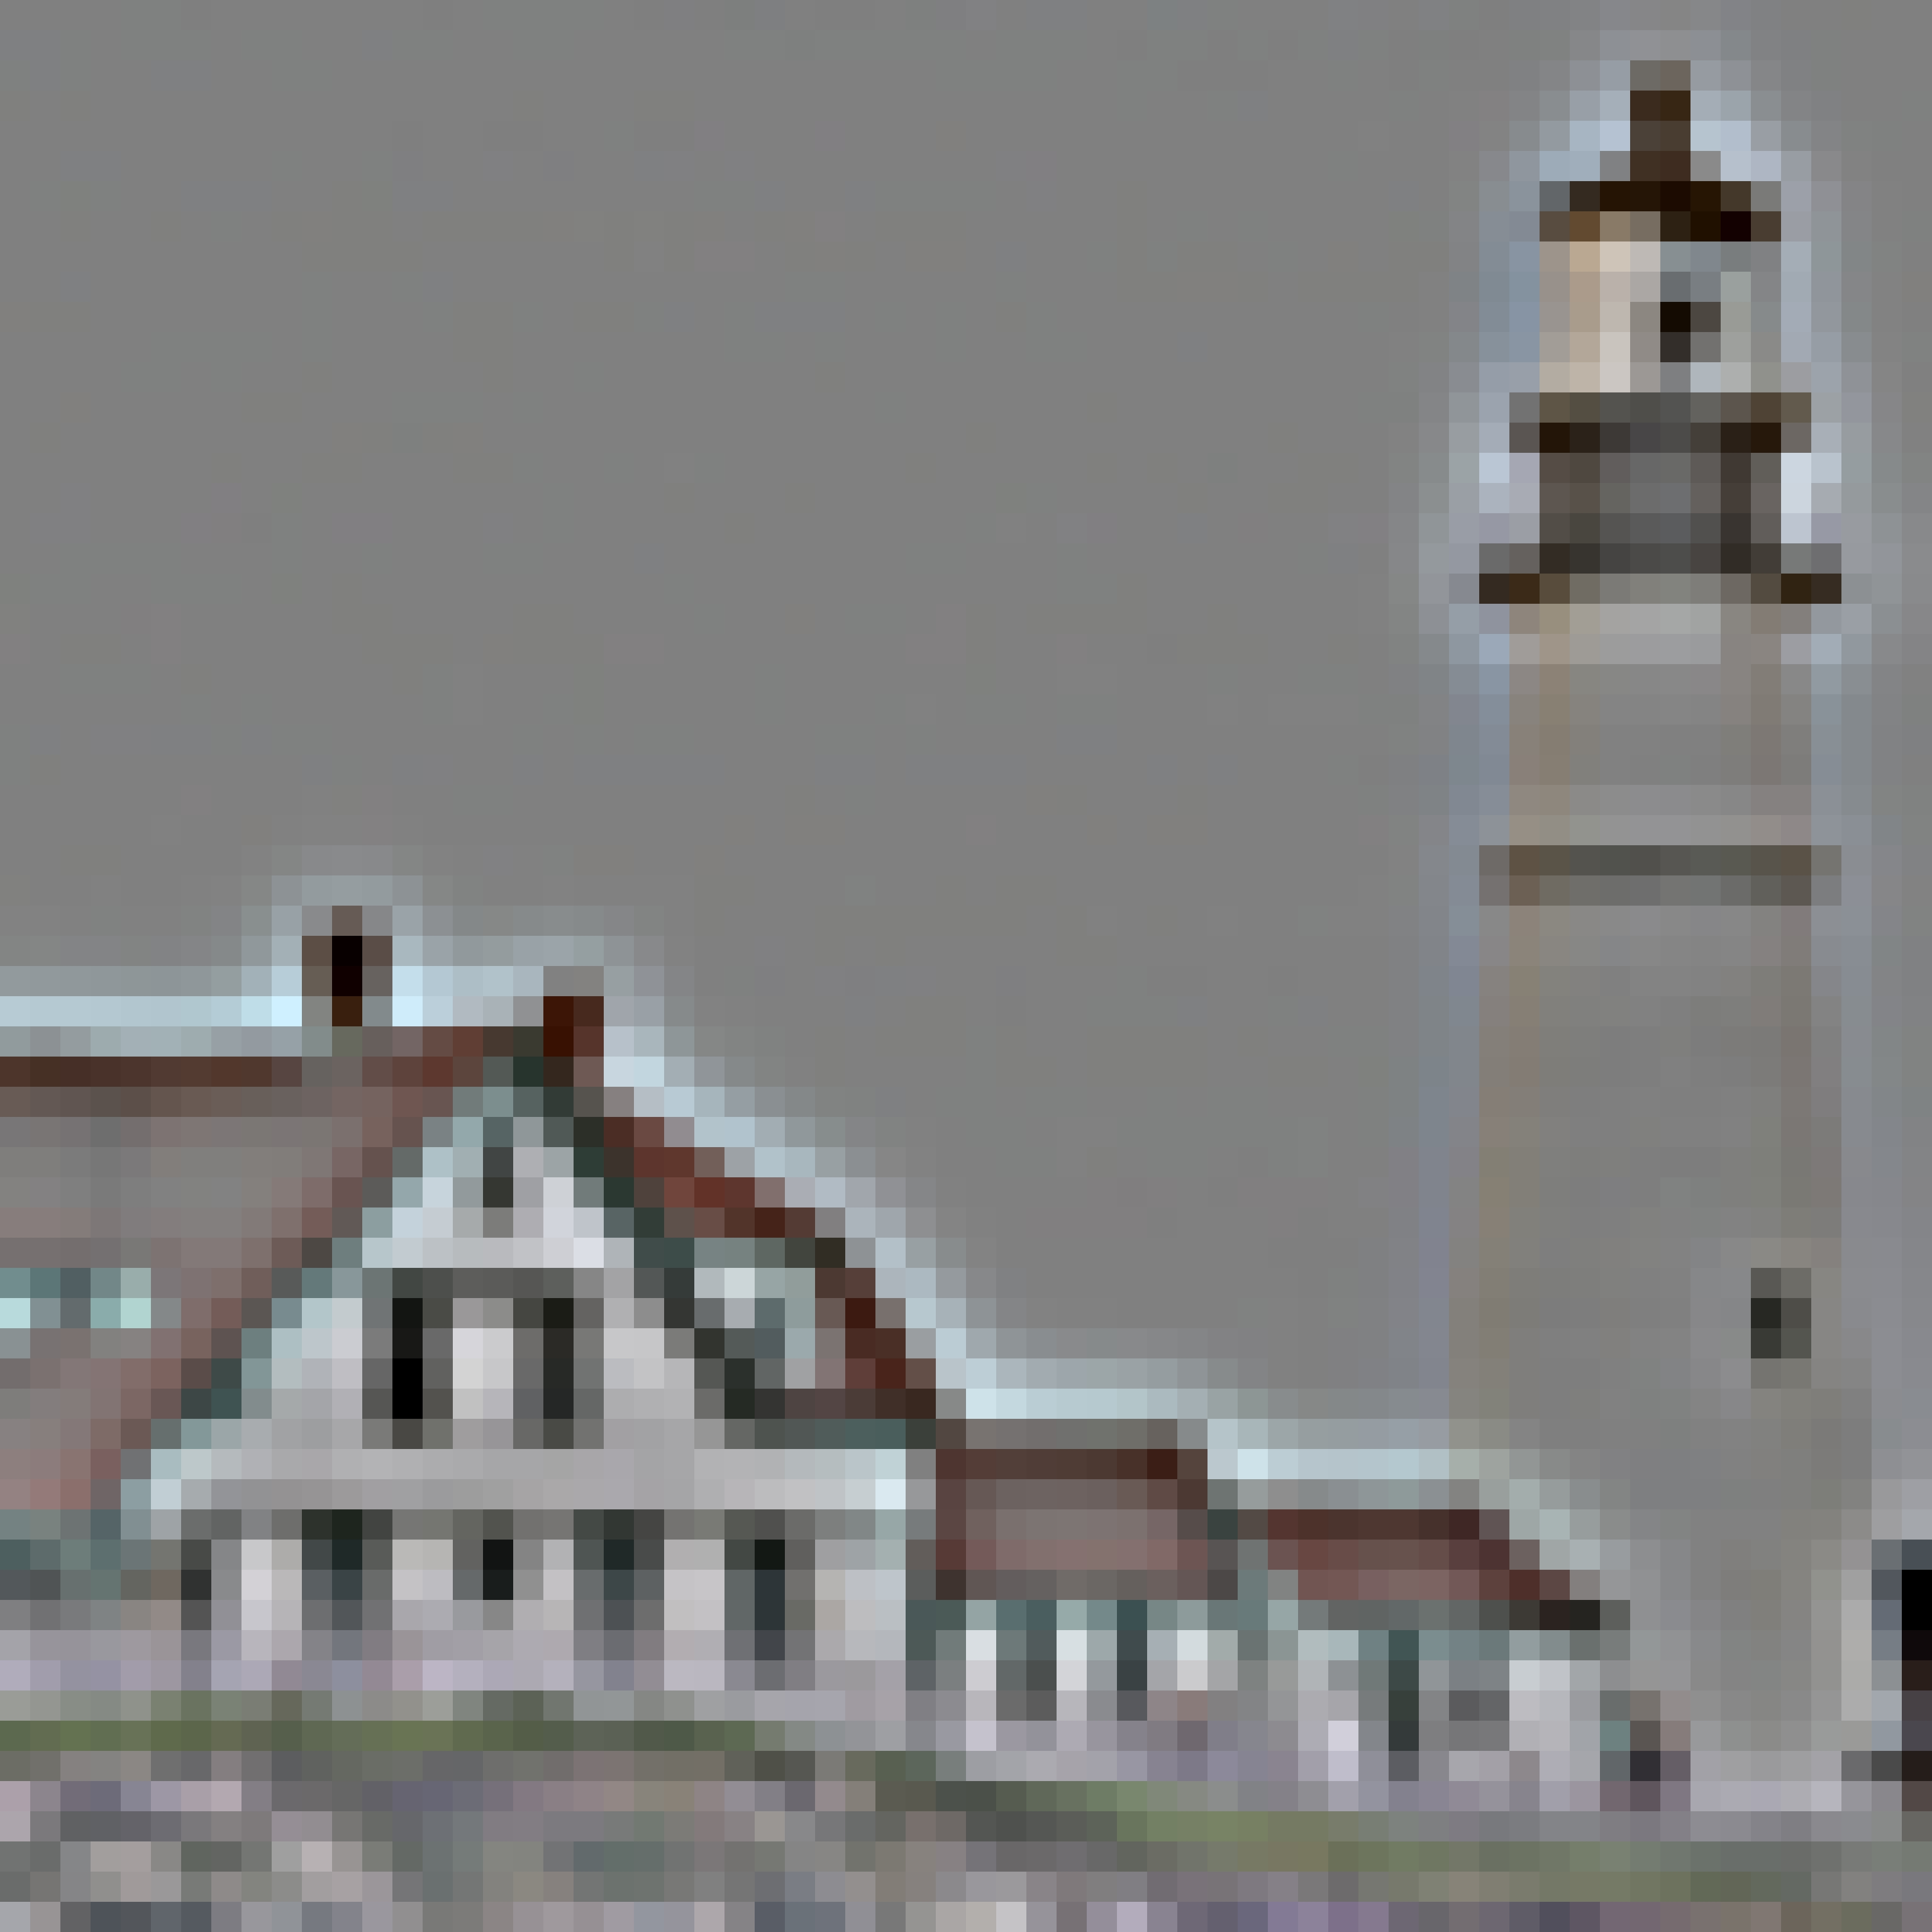
\includegraphics[width=0.12\linewidth]{figures/pyramids/laplacianPyr_3.jpg}
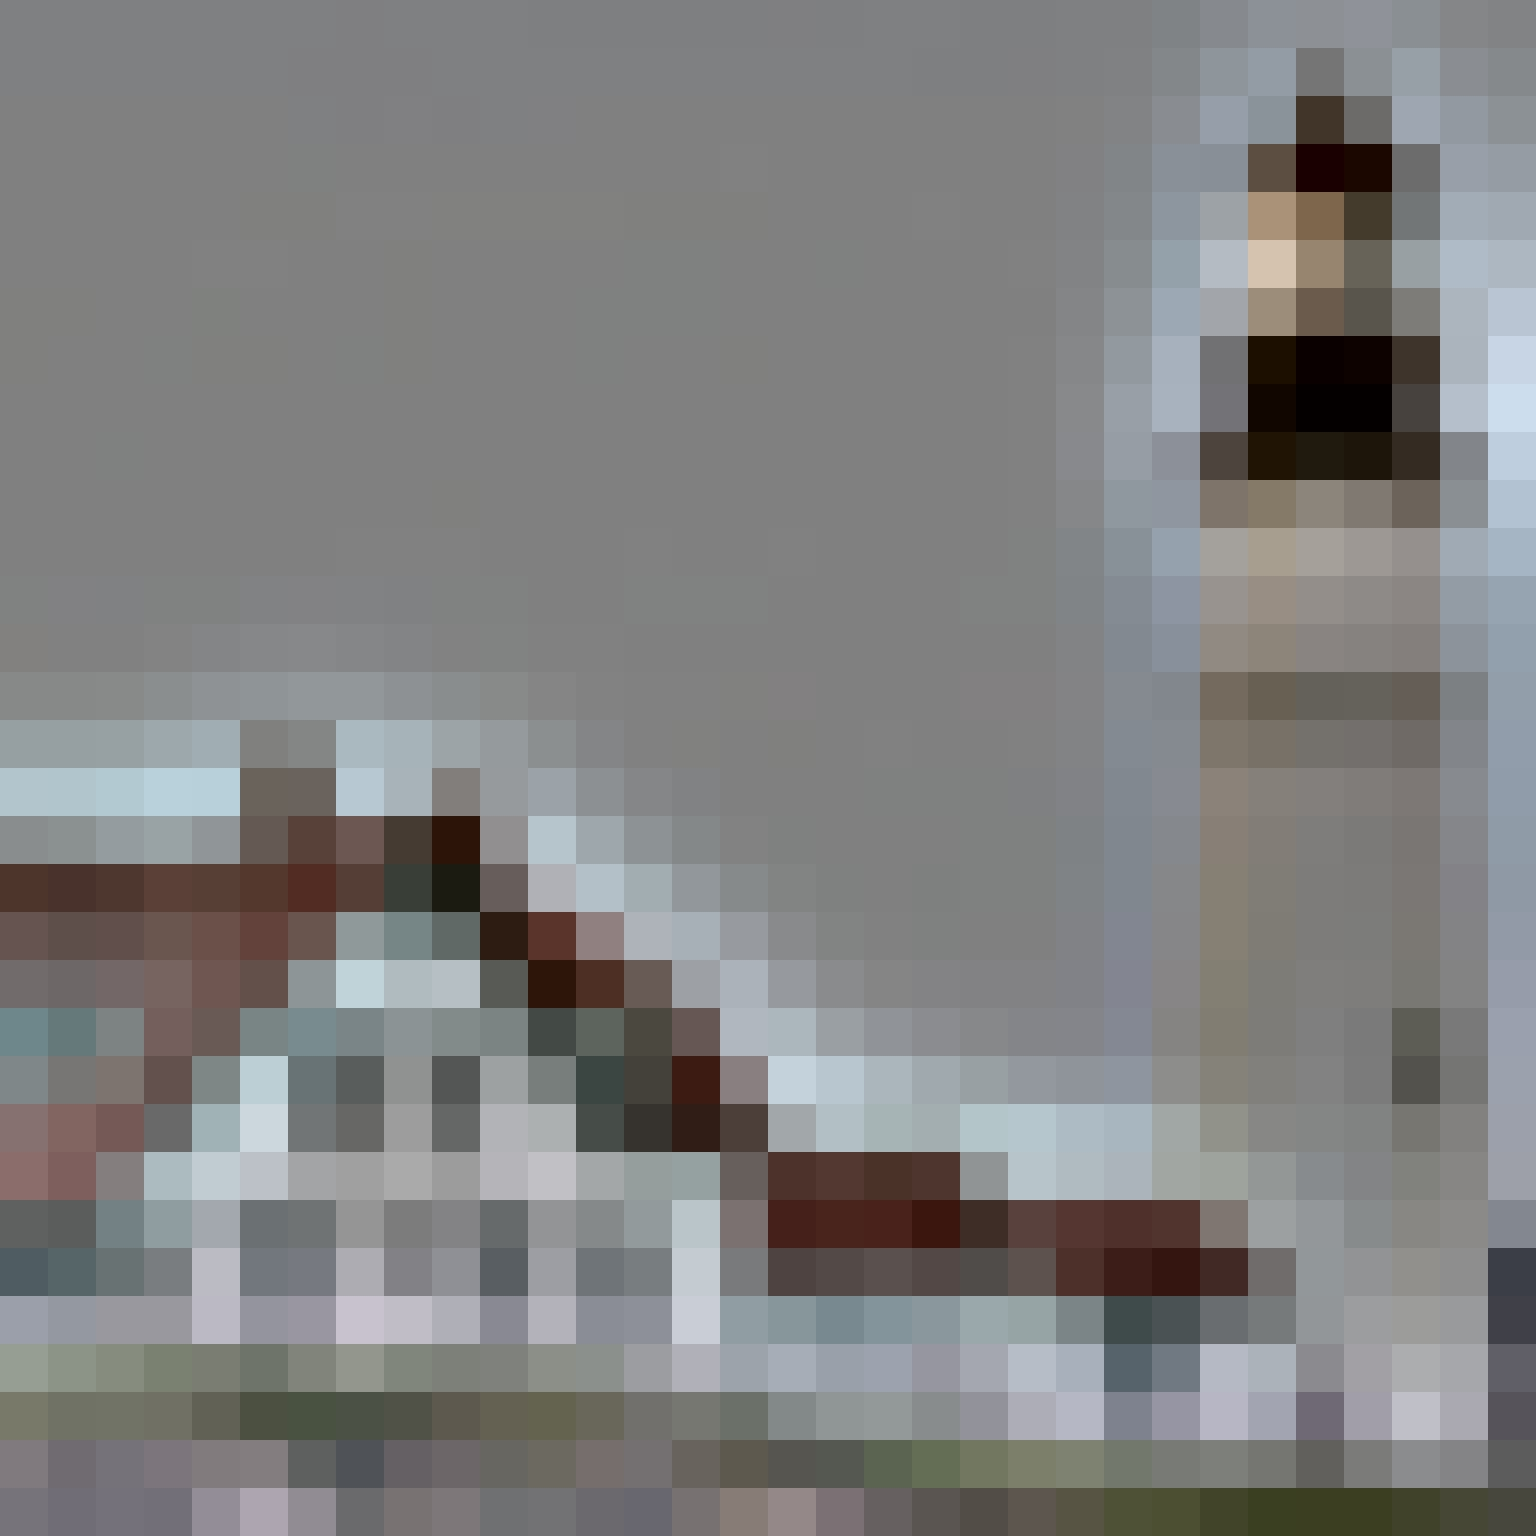
\includegraphics[width=0.06\linewidth]{figures/pyramids/laplacianPyr_4.jpg}
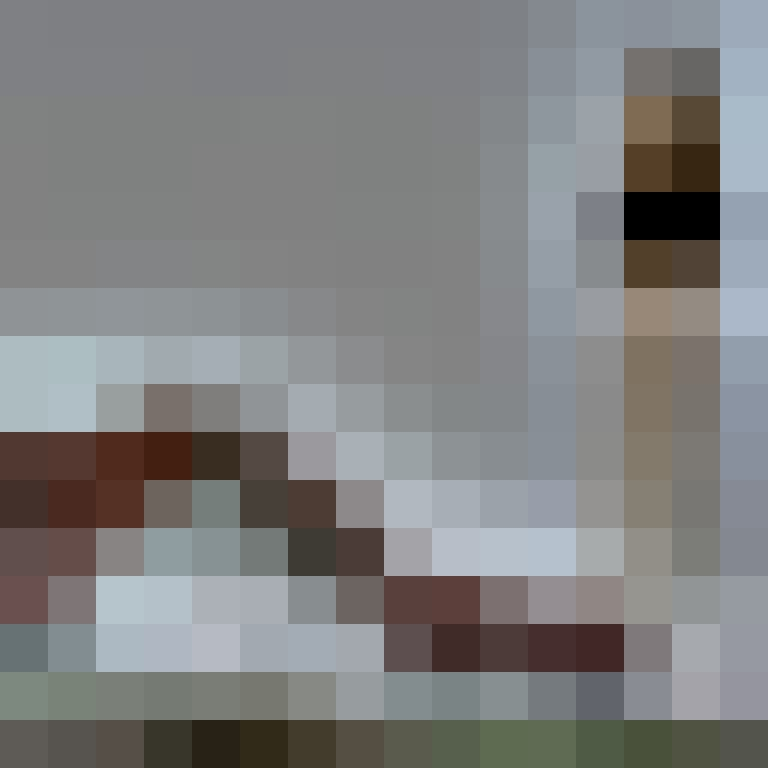
\includegraphics[width=0.03\linewidth]{figures/pyramids/laplacianPyr_5.jpg}

\includegraphics[width=0.015\linewidth]{figures/pyramids/gaussianPyr_6.jpg}
}
\caption{Laplacian pyramid, including the tiny low-pass residual as the last image.  
The Laplacian pyramid is built for each color channel independently.  
%For visualization, we add 128 to all the images. Therefore, the average gray level corresponds to the zero intensity value.
}
\label{fig:laplacpyr}
\end{figure}


Let's write down the matrices in \eqn{\ref{eqn:laplacian_pyr_coef}} for a 1D input $\boldimg$ of length 8, and assuming zero boundary conditions. The operators to compute the first level ($k=0$) of the Laplacian pyramid are:
\begin{equation}
\mathbf{F}_0 =  2 \mathbf{B}_0 \mathbf{U}_0 =
 \frac{1}{8}
 \begin{bmatrix}
  6 ~& 4 ~& 1 ~& 0 ~& 0 ~& 0 ~& 0 ~& 0 \\
  4 ~& 6 ~& 4 ~& 1 ~& 0 ~& 0 ~& 0 ~& 0 \\
  1 ~& 4 ~& 6 ~& 4 ~& 1 ~& 0 ~& 0 ~& 0 \\
  0 ~& 1 ~& 4 ~& 6 ~& 4 ~& 1 ~& 0 ~& 0 \\
  0 ~& 0 ~& 1 ~& 4 ~& 6 ~& 4 ~& 1 ~& 0 \\
  0 ~& 0 ~& 0 ~& 1 ~& 4 ~& 6 ~& 4 ~& 1 \\
  0 ~& 0 ~& 0 ~& 0 ~& 1 ~& 4 ~& 6 ~& 4 \\
  0 ~& 0 ~& 0 ~& 0 ~& 0 ~& 1 ~& 4 ~& 6 
\end{bmatrix}
 \begin{bmatrix}
  1 ~& 0 ~& 0  ~& 0\\
  0 ~& 0 ~& 0  ~& 0\\
  0 ~& 1 ~& 0  ~& 0\\
  0 ~& 0 ~& 0  ~& 0\\
  0 ~& 0 ~& 1  ~& 0\\
  0 ~& 0 ~& 0  ~& 0\\
  0 ~& 0 ~& 0  ~& 1\\
  0 ~& 0 ~& 0  ~& 0
\end{bmatrix}
 \end{equation}
The factor 2 is necessary because inserting zeros decreases the average value of the signal $\mathbf{g}_{k+1}$ by a factor of 2. Multiplying the two matrices:
\begin{equation}
\mathbf{l}_{0} = \mathbf{g}_0 - \mathbf{F}_0 \mathbf{g}_{1} = 
 \mathbf{g}_0 - \frac{1}{8}
 \begin{bmatrix}
  6 ~& 1 ~& 0  ~& 0\\
  4 ~& 4 ~& 0  ~& 0\\
  1 ~& 6 ~& 1  ~& 0\\
  0 ~& 4 ~& 4  ~& 0\\
  0 ~& 1 ~& 6  ~& 1\\
  0 ~& 0 ~& 4  ~& 4\\
  0 ~& 0 ~& 1  ~& 6\\
  0 ~& 0 ~& 0  ~& 4
\end{bmatrix}
 \mathbf{g}_{1}
 \end{equation}
We can also calculate the matrix that should be applied to the input $\boldimg=\mathbf{g_0}$.
\begin{equation}
\mathbf{l}_{0} =  (\mathbf{I} - \mathbf{F}_0 \mathbf{G}_0) \mathbf{g}_0= 
\frac{1}{256}
 \begin{bmatrix}
   182 ~& -56  ~& -24 ~&   -8   ~& -2  ~&   0  ~&   0  ~&   0\\
   -56  ~& 192  ~& -56 ~&  -32   ~& -8   ~&  0  ~&   0   ~&  0\\
   -24  ~& -56  ~& 180  ~& -56 ~&  -24  ~&  -8  ~&  -2   ~&  0\\
    -8   ~&-32  ~& -56  ~& 192  ~& -56  ~& -32  ~&  -8   ~&  0\\
    -2   ~& -8 ~&  -24  ~& -56 ~&  180 ~&  -56  ~& -24 ~&   -8\\
     0   ~&  0  ~&  -8  ~& -32 ~&  -56  ~& 192  ~& -56  ~& -32\\
     0   ~&   0  ~&  -2  ~&  -8  ~& -24  ~& -56 ~&  182  ~& -48\\
     0   ~&   0   ~&  0  ~&   0   ~& -8  ~& -32 ~&  -48 ~&  224
\end{bmatrix}
\boldimg
\end{equation}





Interestingly, the Laplacian pyramid is an invertible transform, but only if we keep the low-pass residual.  We can reconstruct the original image from the Laplacian pyramid. Using the {\bf low-pass residual} signal associated with the Laplacian
pyramid, we can recursively reconstruct the corresponding Gaussian pyramid.  Remember that in the Gaussian pyramid level 1 is just the original image itself, so we can use this to reconstruct the original image
from the Laplacian pyramid. We can do it recursively applying, from $k=N-1$ to $k=0$:
\begin{equation}
\mathbf{g}_k = \mathbf{l}_k + \mathbf{F}_k \mathbf{g}_{k+1}
\label{eq:laplaceRecursion}
\end{equation}

The diagram in \fig{\ref{fig:laplacian_pyr_architecture}} shows the Gaussian pyramid, the Laplacian pyramid and the Laplacian inversion for a three-level Laplacian pyramid. The reconstruction uses the Laplacian pyramid $\mathbf{l}_0,\mathbf{l}_1,...,\mathbf{l}_2$ and the low pass residual $\mathbf{g}_3$ to recover the input signal $\boldimg=\mathbf{g}_0$.

% Definition of blocks:
\begin{figure}[h!]
\centerline{
\tikzset{
  block/.style    = {draw, thin, rectangle, minimum height = 1.5em,  minimum width = 1.5em},
  sum/.style      = {draw, circle, minimum size=.4cm}, % Adder
  input/.style    = {coordinate}, % Input
  output/.style   = {coordinate} % Output
  %x/.style   = {coordinate} % Output
}
\begin{tikzpicture}[auto, thin, node distance=.8cm, >=latex]%triangle 45]
% Drawing the blocks of first level:
\draw
	node [input] (x0) {}
	node [right of=x0, node distance=0.5cm] (x0p) {$\mathbf{g}_0$}
	%node [input] (x0p) {$\mathbf{x}_0$}
	node [block, right of=x0p] (g0) {$\mathbf{G}_0$}
         node [block, red, below of=g0] (f0) {$\mathbf{F}_0$}
	node [sum, red, left of=f0] (suma0) {}
	node [right of=g0] (x1) {$\mathbf{g}_1$}
	node [red, below of=suma0, node distance=2cm] (l0) {$\mathbf{l}_0$};
       % Joining blocks. 
	\draw[-](x0) -- node {} (x0p);
	\draw[->](x0p) -- node {} (g0);
	\draw[->,red](x0p) -- node[pos=0.99, left] {{\tiny $+$}} (suma0);
	\draw[->,red](f0) -- node[pos=0.99, below] {{\tiny $-$}} (suma0);
	\draw[->,red](x1) |- node {} (f0);
	\draw[-](g0) |- node {} (x1);
	\draw[->,red](suma0) -- node {} (l0);

\draw
	node [input,right of=x1, node distance=.8cm] (x1p) {}
	%node [input] (x0p) {$x_0$}
	node [block, right of=x1p] (g1) {$\mathbf{G}_1$}
    node [block, red, below of=g1] (f1) {$\mathbf{F}_1$}
	node [sum, red, left of=f1] (suma1) {}
	node [right of=g1] (x2) {$\mathbf{g}_2$}
	node [red, below of=suma1, node distance=1.5cm] (l1) {$\mathbf{l}_1$};
       % Joining blocks. 
	\draw[-](x1) -- node {} (x1p);
	\draw[->](x1p) -- node {} (g1);
	\draw[->,red](x1p) -- node[pos=0.99, left] {{\tiny $+$}} (suma1);
	\draw[->,red](f1) -- node[pos=0.99, below] {{\tiny $-$}} (suma1);
	\draw[->,red](x2) |- node {} (f1);
	\draw[-](g1) |- node {} (x2);
	\draw[->,red](suma1) -- node {} (l1);
	
\draw
	node [input,right of=x2, node distance=.8cm] (x2p) {}
	node [block, right of=x2p] (g2) {$\mathbf{G}_2$}
        node [block, red, below of=g2] (f2) {$\mathbf{F}_2$}
	node [sum, red, left of=f2] (suma2) {}
	node [right of=g2] (x3) {$\mathbf{g}_3$}
	node [red, below of=suma2, node distance=1cm] (l2) {$\mathbf{l}_2$};
       % Joining blocks. 
	\draw[-](x2) -- node {} (x2p);
	\draw[->](x2p) -- node {} (g2);
	\draw[->,red](x2p) -- node[pos=0.99, left] {{\tiny $+$}} (suma2);
	\draw[->,red](f2) -- node[pos=0.99, below] {{\tiny $-$}} (suma2);
	\draw[->,red](x3) |- node {} (f2);
	\draw[-](g2) |- node {} (x3);
	\draw[->,red](suma2) -- node {} (l2);

\draw
	node [block, blue, right of=x3] (f4) {$\mathbf{F}_2$}
	node [sum, blue, right of=f4] (suma4) {{\tiny $+$}}
	node [block, blue, right of=suma4] (f5) {$\mathbf{F}_1$}
	node [sum, blue, right of=f5] (suma5) {{\tiny $+$}}
	node [block, blue, right of=suma5] (f6) {$\mathbf{F}_0$}
	node [sum, blue, right of=f6] (suma6) {{\tiny $+$}}
	node [input, blue, right of=suma6] (rx) {};
	\draw[->,blue](x3) -- node {} (f4);
	\draw[->,blue](f4) -- node {} (suma4);
	\draw[->,blue](suma4) -- node {} (f5);
	\draw[->,blue](f5) -- node {} (suma5);
	\draw[->,blue](suma5) -- node {} (f6);
	\draw[->,blue](f6) -- node {} (suma6);
	\draw[->,blue](suma6) -- node {} (rx);
	
% reconstruction arrows
	\draw[->,blue](l0) -| node {} (suma6);
	\draw[->,blue](l1) -| node {} (suma5);
	\draw[->,blue](l2) -| node {} (suma4);
\end{tikzpicture}
}
\caption{The diagram shows the Gaussian pyramid (black), the Laplacian pyramid (red) and the Laplacian inversion for a three-level Laplacian pyramid (blue).}
\label{fig:laplacian_pyr_architecture}
\end{figure}





This architecture has two parts: (1) the analysis network (or {\bf encoder}) that transforms the input image $\mathbf{x}$ into a representation composed of $\mathbf{l}_0, \mathbf{l}_1, ...$ and the low pass residual $\mathbf{x}_n$; and (2) the synthesis network (or {\bf decoder}) that reconstructs the input from the representation.  The Laplacian pyramid is an {\bf overcomplete representation}
\index{Overcomplete representation}
(more coefficients than pixels); the dimensionality of the representation is higher than the dimensionality of the input.
\marginnote{{\bf Encoder} and {\bf decoder} networks are also common building blocks of deep neural networks.%, as we will see in Chapter XX. 
The Laplacian pyramid can be considered as a special type of deep neural net.}[-1.0cm]

Note that the reconstruction property of the Laplacian pyramid does not depend on the filters used for subsampling and upsampling. Even if we used random filters the reconstruction property would still hold. 

%The Laplacian pyramid is used in many image processing applications.  In the next section we show one fun application: {\bf image blending}.

\subsection{Image Blending}

Image blending (or image compositing) consists in introducing elements of one image inside another. Creating convincing composite images is challenging, as the edge between the two images has to be invisible. One way of formalizing the image-blending operation is by defining a mask, $\mathbf{m}$, that specifies how the images will be combined. The mask is used to select which pixels come from each of the two images in order to create the composite image. For example, let's blend two images using the mask as shown in \fig{\ref{fig:orange_apple_mask}}.

\begin{figure}[h!]
\centerline{
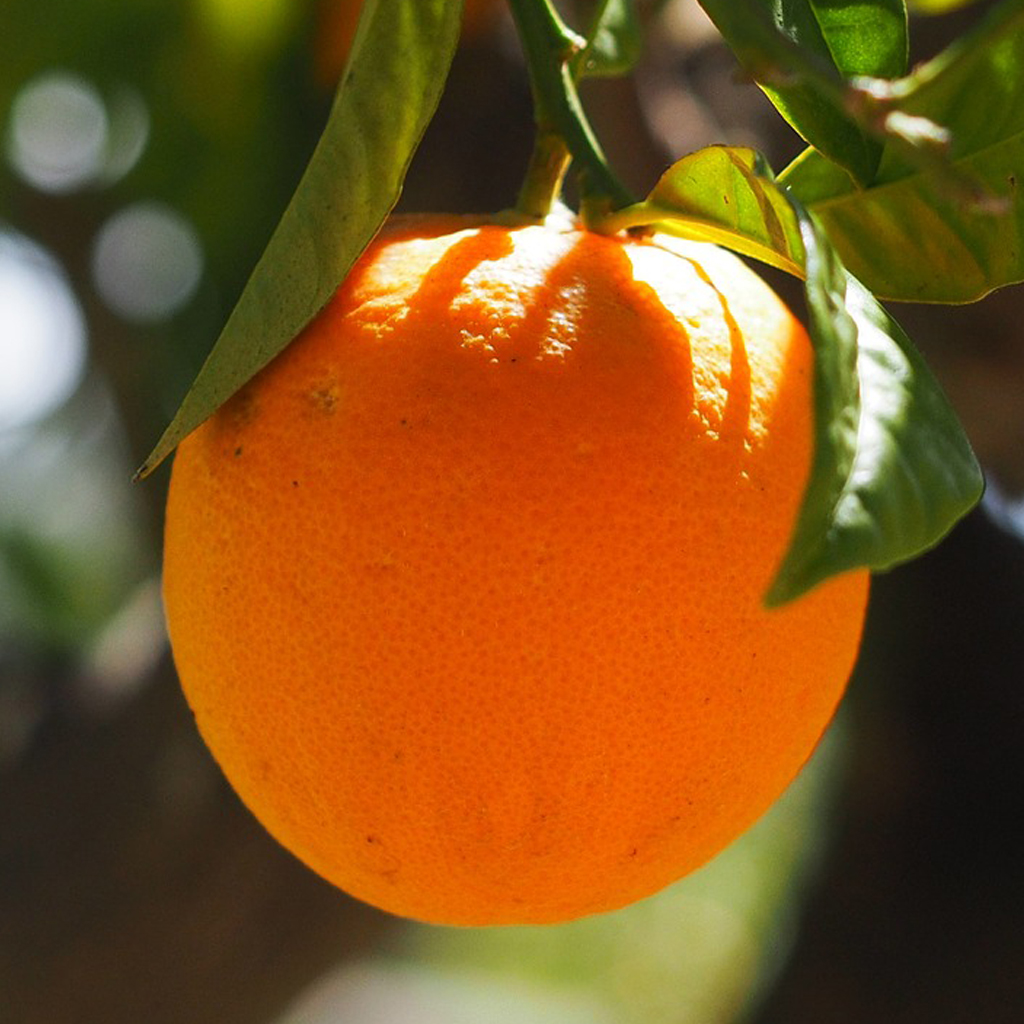
\includegraphics[width=0.30\linewidth]{figures/pyramids/orange.jpg}
~
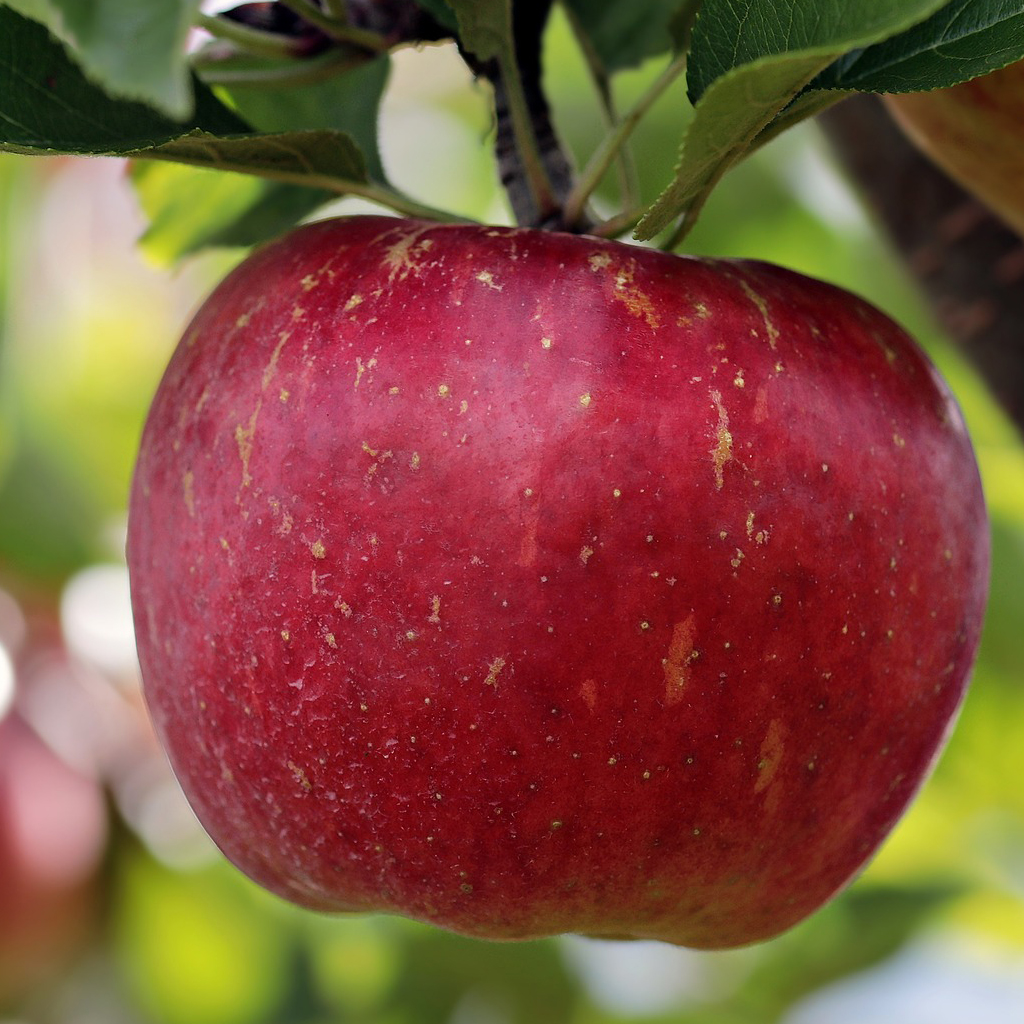
\includegraphics[width=0.30\linewidth]{figures/pyramids/apple.jpg}
~

\includegraphics[width=0.30\linewidth]{figures/pyramids/mask10_b.jpg}
}
\caption{Two images to be blended and the blending mask.}
\label{fig:orange_apple_mask}
\end{figure}

%The Laplacian pyramid is used in many image processing or analysis
%applications.  Here we show one fun application:  image blending
%(you'll do this in a homework problem).  
In this example, the mask indicates that the blended image will combine the half-left of the first image with the right-half of the second image. One naive solution to this problem will be to define blending as $\boldimgout = \boldimg^A * \mathbf{m} + \boldimg^B * (1-\mathbf{m})$, giving as result the image in \fig{\ref{fig:orange_apple_mask_bad_result}}.

\begin{figure}[h!]
\centerline{
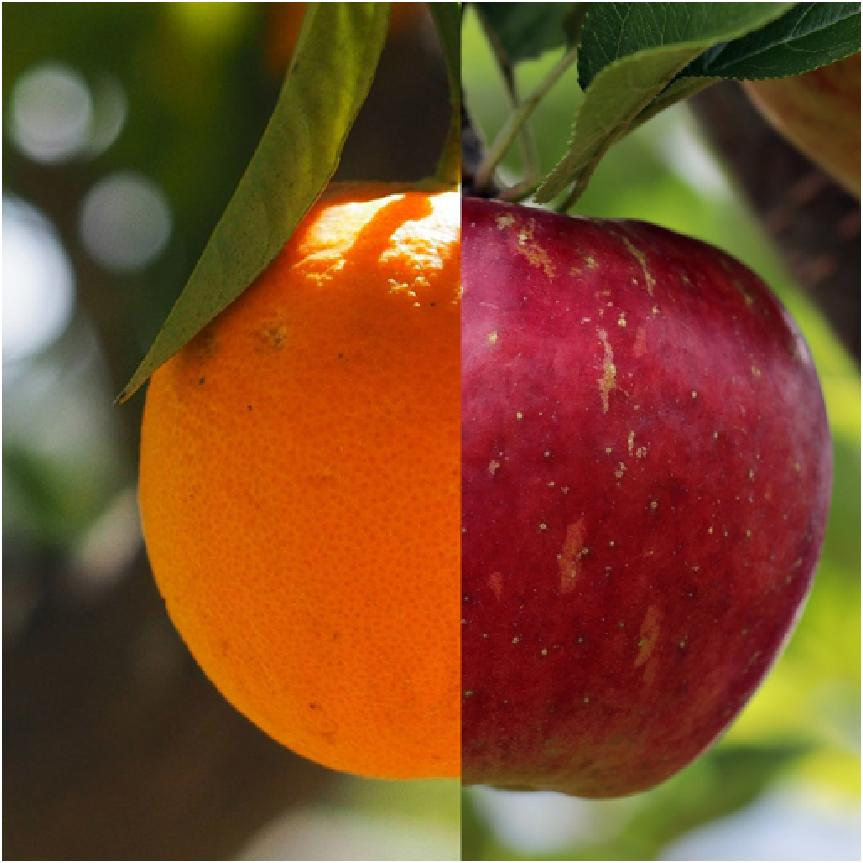
\includegraphics[width=0.30\linewidth]{figures/pyramids/apple_orange_mask_8levels.jpg}
}
\caption{Resulting blended image from \fig{\ref{fig:orange_apple_mask}}. This result is not very pleasing.}
\label{fig:orange_apple_mask_bad_result}
\end{figure}

The result in \fig{\ref{fig:orange_apple_mask_bad_result}} is not very pleasing as there is a sharp transition from one image to another (see the straight edge between the two halves of the apple and orange.) We would like to be able to merge both images in a seamless way. In 1983, Burt and Adelson \cite{Burt83} introduced an image blending algorithm using Laplacian pyramid capable of achieve a smooth transition between the two images. This approach remains one of the best solutions to this problem.

Using the Laplacian pyramid, we can transition from one image to the next over many different spatial scales to make a gradual transition between the two images. The algorithm proceeds as follows. We first build the Laplacian pyramid for the two input images; in this example we use seven levels and we also keep the last low-pass residual as shown in \fig{\ref{fig:blending_pyrs}}.

\begin{figure}[h!]
\centerline{
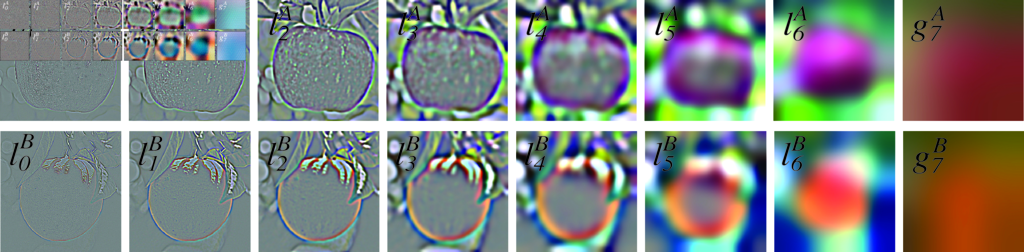
\includegraphics[width=0.9\linewidth]{figures/pyramids/blending_pyrs.eps}
}
\caption{Laplacian pyramids (seven levels and Gaussian residual) for both input images.}
\label{fig:blending_pyrs}
\end{figure}

The second step is to build the Gaussian pyramid of the mask as shown in \fig{\ref{fig:blending_pyrs_mask}} (note that we use eight levels, one level more than for the Laplacian pyramid).
\begin{figure}[h!]
\centerline{
\includegraphics[width=0.9\linewidth]{figures/pyramids/blending_pyrs_mask.eps}
}
\caption{Gaussian pyramid of the mask.}
\label{fig:blending_pyrs_mask}
\end{figure}

%as shown in the apple/orange in the bottom right of Fig.~\ref{fig:appleorange}. 
%To do this, both images are analyzed first by the Laplacian pyramid. The mask is analyzed by the Gaussian pyramid. 
In the third step, we combine the three pyramids to compute the Laplacian pyramid of the blended image. The Laplacian pyramid of the blended image is obtained as 
\begin{equation}
\mathbf{l}_k = \mathbf{l}_k^A * \mathbf{m}_k + \mathbf{l}_i^B * (1-\mathbf{m}_k)
\end{equation}
The same is done for the low-pass residual. 

Finally, the fourth step consists in collapsing (i.e., decoding) the resulting pyramid to produce the blended image shown in \fig{\ref{fig:appleorange}}.

\begin{figure}[h!]
%\centerline{
%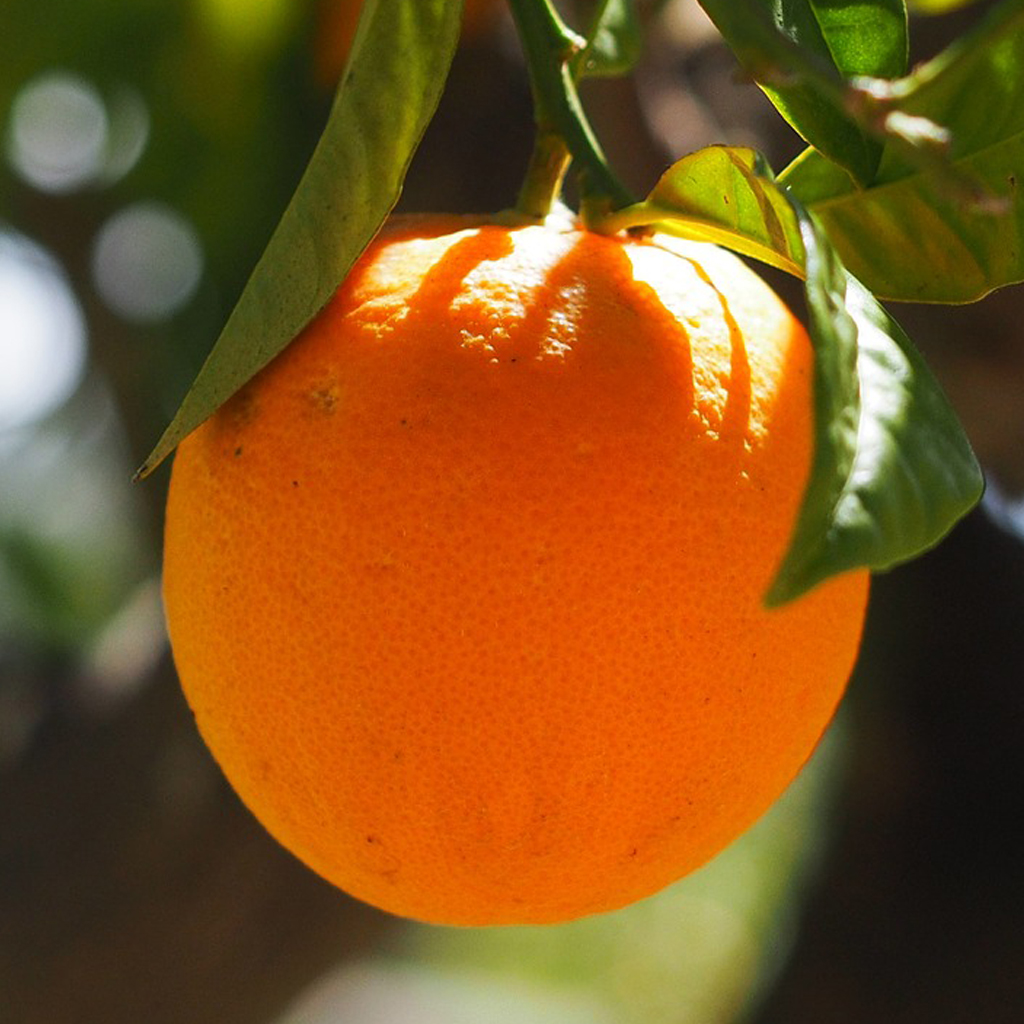
\includegraphics[width=0.3\linewidth]{figures/pyramids/orange.jpg}
%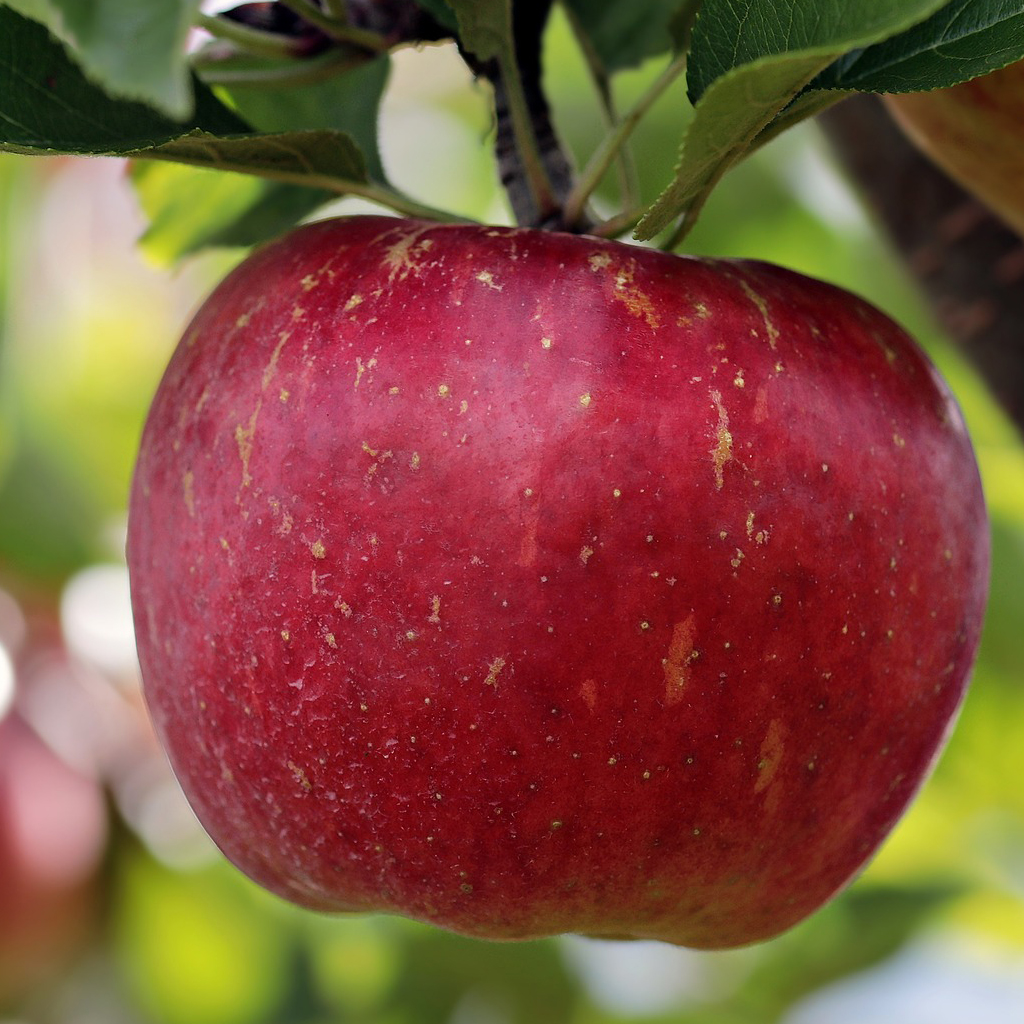
\includegraphics[width=0.3\linewidth]{figures/pyramids/apple.jpg}
%
\includegraphics[width=0.3\linewidth]{figures/pyramids/mask10.jpg}
%}
%\centerline{
%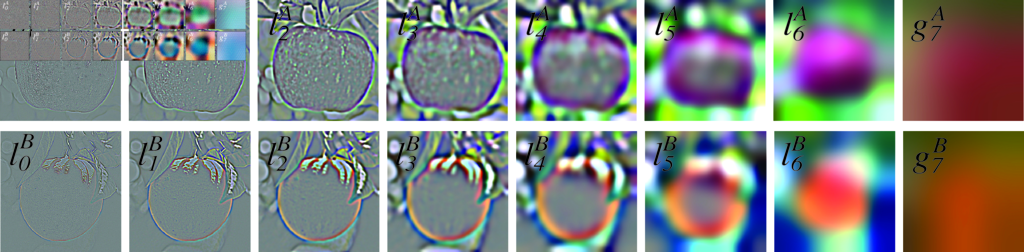
\includegraphics[width=0.9\linewidth]{figures/pyramids/blending_pyrs.eps}
%}
\centerline{
%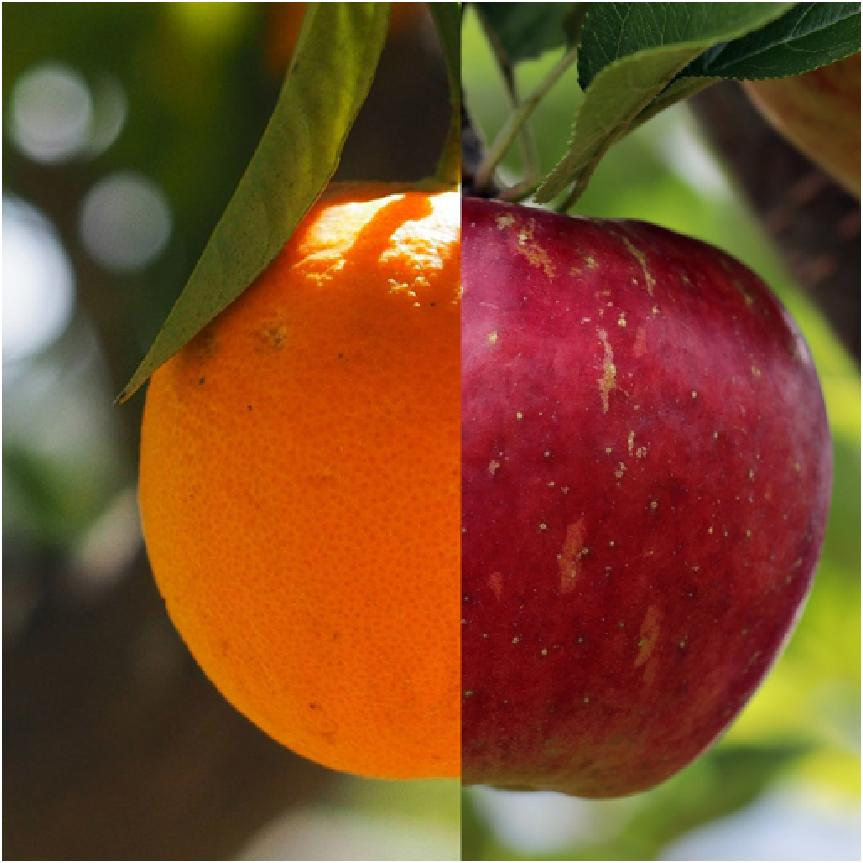
\includegraphics[width=0.45\linewidth]{figures/pyramids/apple_orange_mask_8levels.jpg}
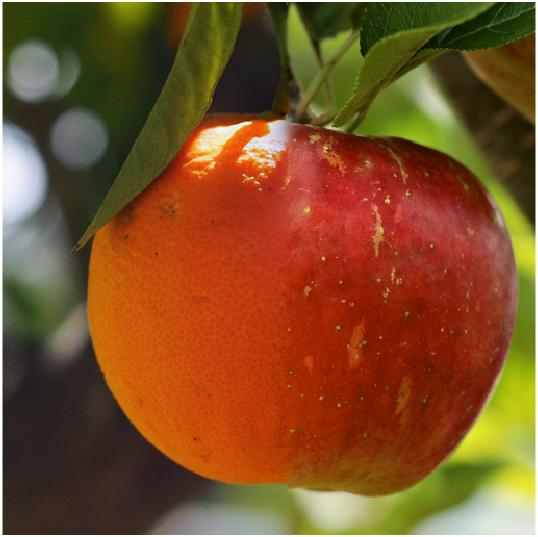
\includegraphics[width=0.35\linewidth]{figures/pyramids/apple_orange_laplacian_8levels.jpg}
}
\caption{Image compositing with the Laplacian pyramid. Example inspired by \cite{Burt83}.}
\label{fig:appleorange}
\end{figure}

The result in \fig{\ref{fig:appleorange}} has a smooth transition between the two sides and produces a pleasing blending. The mask does no need to be rectangular. It is possible to blend arbitrary images with complex masks, but the quality of the final image will depend on how well aligned the images are and the composition of the objects in the scene. 
This is method remains one of the most popular methods for image blending due to its simplicity and the quality of the resulting images. 

\marginnote{This method will fail when blending requires geometric image transformations.}
%
%


%


%
%
%\begin{figure}
%\centerline{
%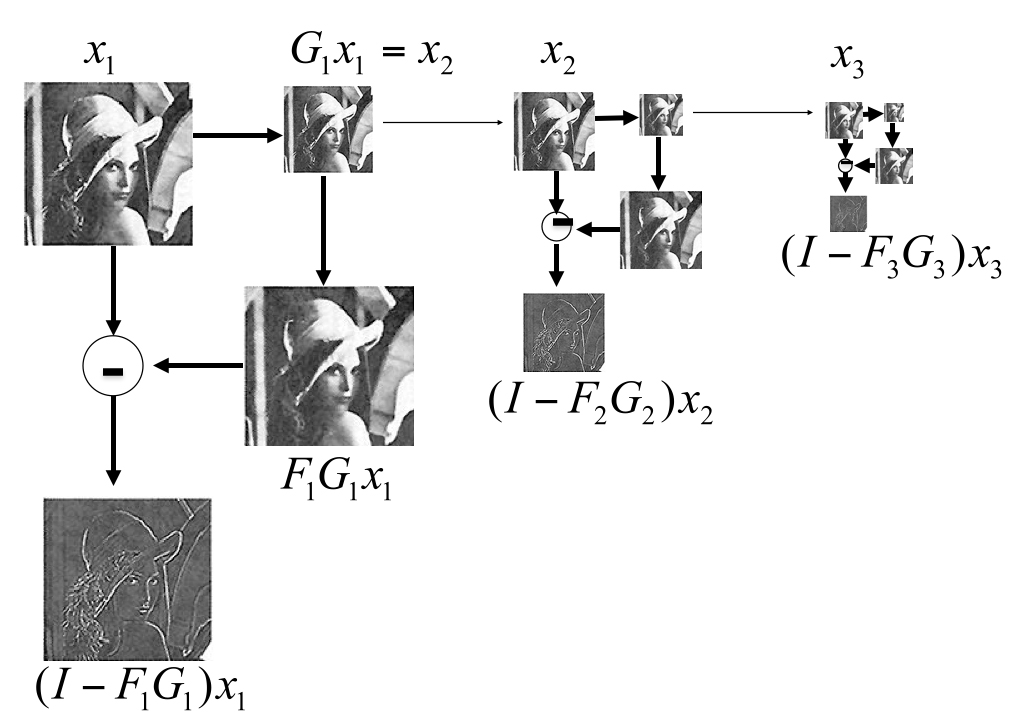
\includegraphics[width=0.5\linewidth]{figures/pyramids/lmat.jpg}
%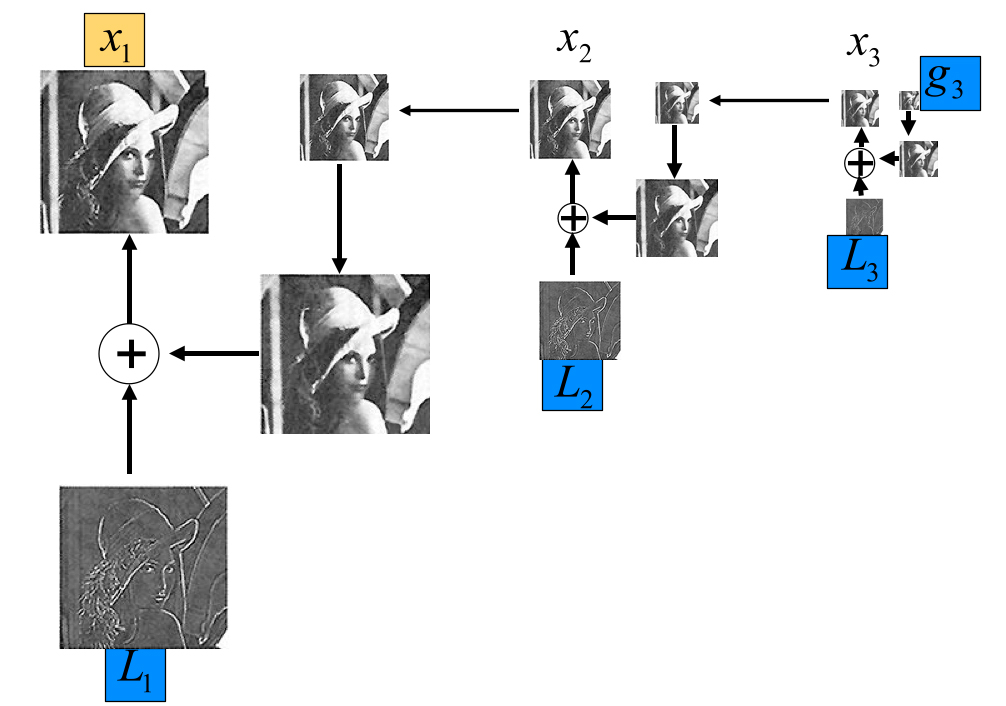
\includegraphics[width=0.5\linewidth]{figures/pyramids/lmatrecon.jpg}
%}
%\caption{Laplacian pyramid construction, and reconstruction from that
%  representation. }
%\label{fig:lmat}
%\end{figure}
%
%
%The Laplacian pyramid is simple:  it represents, at each level, what
%is present in a Gaussian pyramid image of one level, but not present
%at the level below it.  We calculate that by expanding the
%lower-resolution Gaussian pyramid image to the same pixel resolution
%as the neighboring higher-resolution Gaussian pyramid image, then
%subtracting the two.  This calculation is made in a recursive,
%telescoping fashion.  By storing a recursion-ending Gaussian
%low-resolution image, the original image can be reconstructed from its
%Laplacian pyramid representation, Fig.~\ref{fig:lmat}.
%
%
%\begin{figure}
%\centerline{
%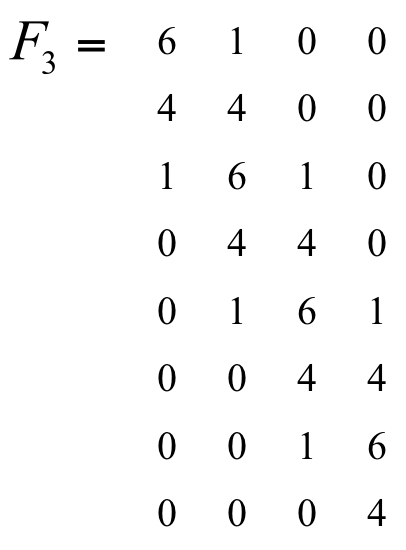
\includegraphics[width=0.2\linewidth]{figures/pyramids/upsamp.jpg}
%}
%\caption{The blur-and-upsample operator, shown for a 1-d signal.  A 2-d
%  implementation can be achieved with the 1-d version applied
%  separably in each dimension. }
%\label{fig:upsamp}
%\end{figure}
%
%%\subsubsection{Laplacian pyramid steps}
%
%Here are the steps for calculating a Laplacian pyramid.  Let the
%operator $G_n$ be the blur-and-downsample operator at pyramid level $n$.
%This is shown in Fig.~\ref{fig:gpnums}.  Let $F_n$ be the
%blur-and-upsample operator for pyramid level $n$, shown in
%Fig.~\ref{fig:upsamp}.   Then the Laplacian pyramid coefficients,
%$L_n$, at pyramid level $n$, are:  
%\begin{equation}
%L_n = (I_n - F_n G_n) x_n,
%\end{equation}
%where $I_n$ is the identity operator for pyramid level $n$, and $x_n$
%is the Gaussian pyramid coefficients for the image at level $n$.
%
%Using the low-pass residual signal associated with the Laplacian
%pyramid, we can recursively reconstruct the corresponding Gaussian
%pyramid.  Remember that Gaussian pyramid level 1 is just the original
%image itself, so we can use this to reconstruct the original image
%from the Laplacian pyramid, with its lowpass residual:
%\begin{equation}
%x_n = L_n + F_n x_{n+1}
%\label{eq:laplaceRecursion}
%\end{equation}
%A repeated applications of Eq.~(\ref{eq:laplaceRecursion}), we can
%recover $x_1$, the original image.
%
%
%\begin{figure}
%\centerline{
%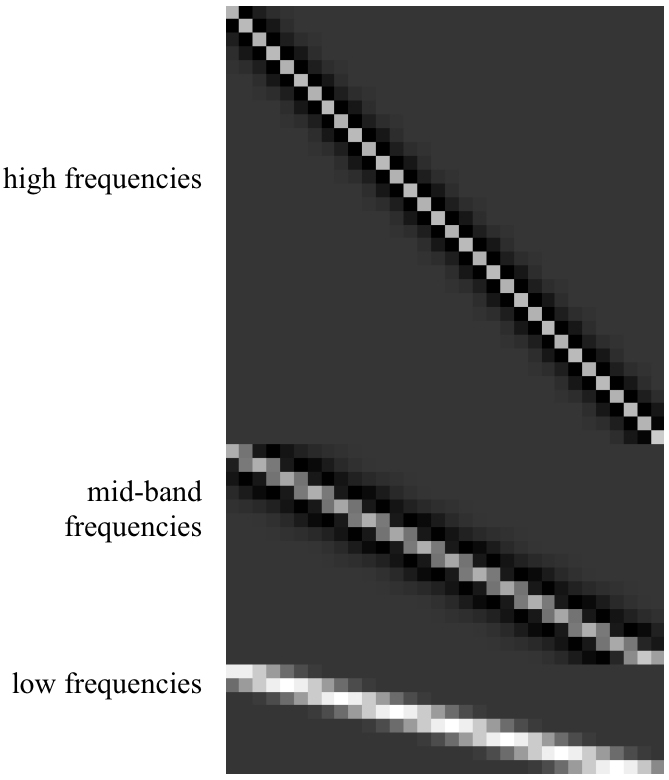
\includegraphics[width=0.4\linewidth]{figures/pyramids/lapmat.jpg}
%}
%\caption{Matrix visualization of Laplacian pyramid. }
%\label{fig:lapmat}
%\end{figure}
%
%Fig.~\ref{fig:lapmat}
% is the equivalent matrix which creates a 1-d Laplacian pyramid
%from an input column vector (again, the actual computation is more
%efficient than is multiplying by this matrix).
%
%\begin{figure}
%\centerline{
%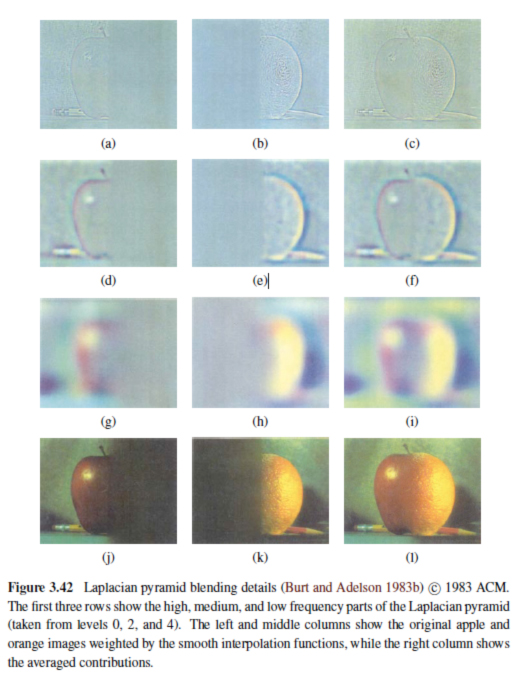
\includegraphics[width=0.55\linewidth]{figures/pyramids/appleLaplace.jpg}
%}
%\caption{Laplacian pyramid for image compositing}
%\label{fig:appleLaplace}
%\end{figure}
%
%
%\subsection{Haar and QMF pyramids}
%
%\subsubsection{1-d Haar transform}
%
%The Laplacian pyramid is an overcomplete representation (more
%coefficients than pixels).  The wavelet (or sometimes called a
%quadrature mirror filter (QMF) pyramid, in the signal processing
%community) transform will be complete (instead of overcomplete), and
%adds some orientation tuning.  The Haar transform is the simplest
%version, yet still has many of the properties of other wavelet
%transforms, so let's derive that first.
%
%Suppose we have the submatrix, U.   The first coefficient of the
%transform is just the average of the two input pixels, and the 2nd
%coefficient it the difference.  Clearly, that's an invertible change
%of basis, and the inverse is shown here as $U^{-1}$.  
%
%
%\begin{figure}
%\centerline{
%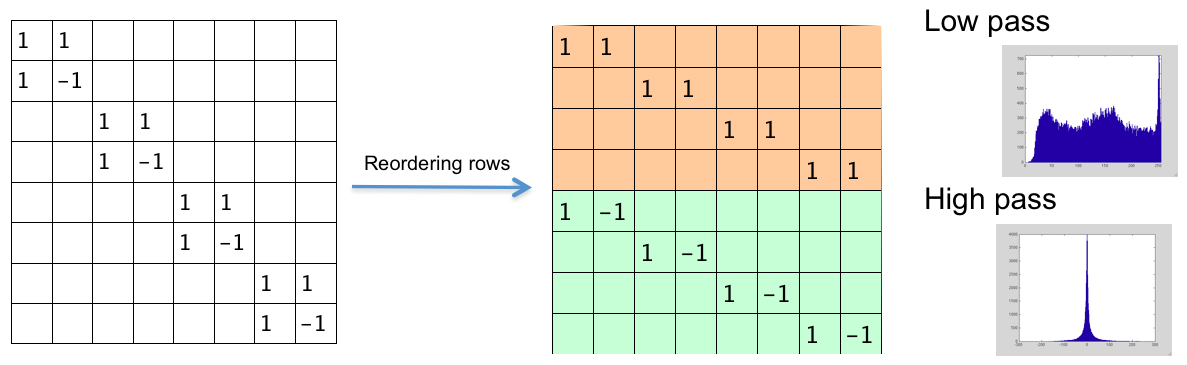
\includegraphics[width=0.7\linewidth]{figures/pyramids/haar1.jpg}
%}
%\centerline{
%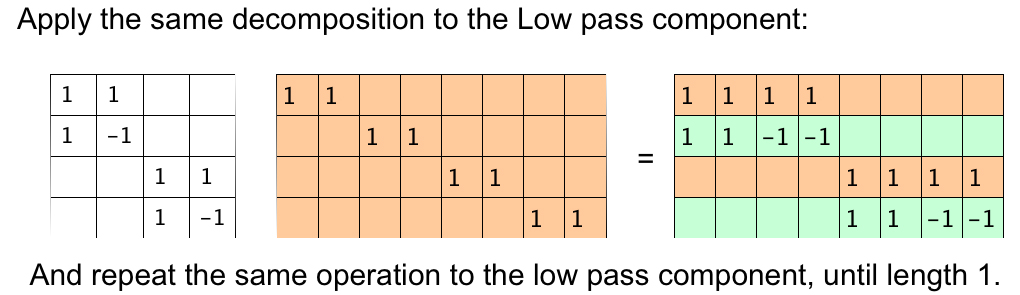
\includegraphics[width=0.7\linewidth]{figures/pyramids/haar2.jpg}
%}
%\caption{Haar wavelet decomposition}
%\label{fig:haar1d1}
%\end{figure}
%
%
%
%
%One thing to note here is the aliasing of each subband,
%and its cancellation when the two subbands are combined.   In both the
%high and the low bands, we're taking every other sample of a signal
%convolved with some two-tap filter.  Those two-tap (high or low-pass)
%filters don't sufficiently pre-filter the signal to avoid aliasing in
%the resulting subsampled signal.  So how do we obtain perfect
%reconstruction from those filter banks?  Each band relies on the other
%one to supply the information needed to removing the aliasing that
%happens from one band alone.  (We can easily see how the other band is
%used for reconstruction in the space-domain view of things.  The
%Fourier domain explanation involves the aliasing components from each band
%that cancel each other.)
%
%We can replicate this submatrix in different subspaces of a larger
%matrix, and re-order the rows to make it obvious that we're creating a
%low-pass version of the signal, and a high-pass one.
%Fig.~\ref{fig:haar1d2} shows another construction of the Haar transform
%matrix, and its inverse.
%
%
%\begin{figure}
%\centerline{
%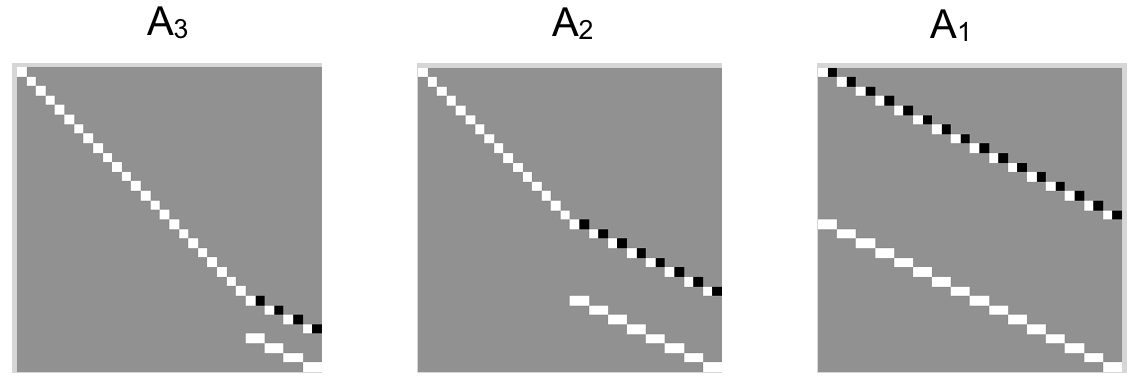
\includegraphics[width=0.7\linewidth]{figures/pyramids/haar3.jpg}
%}
%\centerline{
%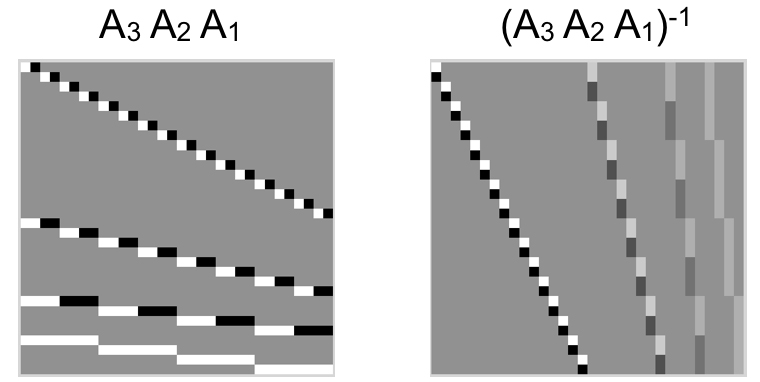
\includegraphics[width=0.5\linewidth]{figures/pyramids/haar4.jpg}
%}
%\caption{more on 1-d haar wavelet}
%\label{fig:haar1d2}
%\end{figure}
%
%\subsubsection{2-d Haar transform}
%
%We apply the 1-d Haar transform separably in 2-d, which leads to:  a
%low-pass band, a vertical high-pass band, a horizontal high-pass band,
%and a ``diagonal'' band, high-pass in both horizontal and vertical.
%Unfortunately, that last band isn't a rotation of either of the other
%two band-pass bands.    The wavelet transform is great for
%compression, since it's ``complete'', with the same number of
%coefficients as pixels.  For the Haar filter, reconstruction from the
%transform domain is exact, but for other filters it is only
%approximate.
%
%The Haar filters are just the simplest
%example of an orthonormal wavelet, or QMF, filter set.  Larger filters
%have only approximate image reconstruction, but have nicer frequency
%localization properties and are generally used instead of the Haar filters.
%
%\begin{figure}
%\centerline{
%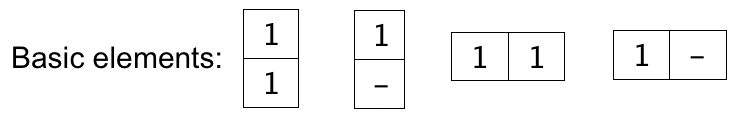
\includegraphics[width=0.4\linewidth]{figures/pyramids/haar2d1.jpg}
%}
%\centerline{
%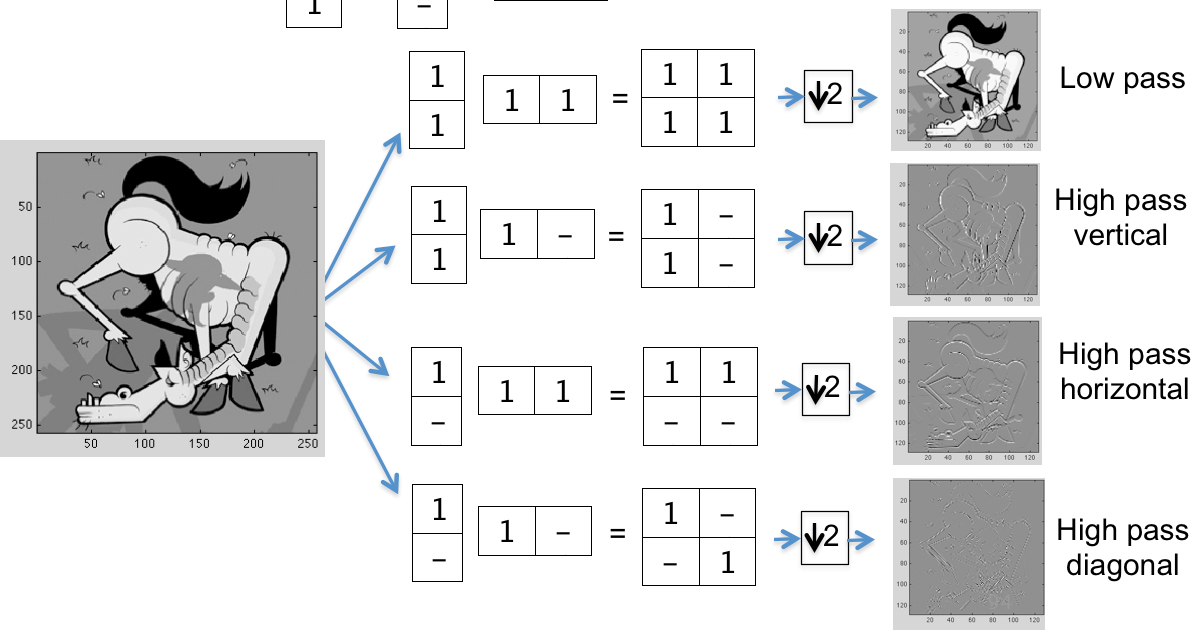
\includegraphics[width=0.8\linewidth]{figures/pyramids/haar2d2.jpg}
%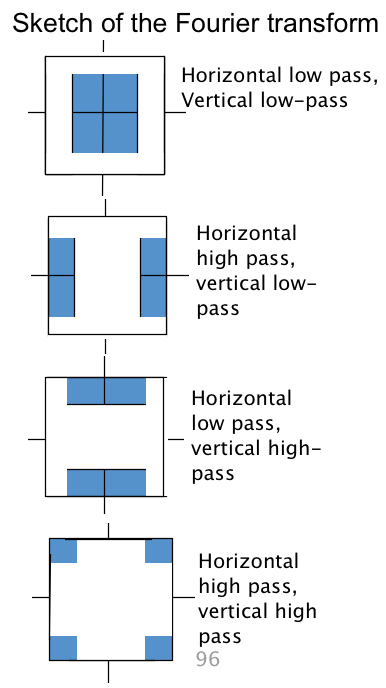
\includegraphics[width=0.24\linewidth]{figures/pyramids/haar2d3.jpg}
%}
%\caption{2d haar wavelet}
%\label{fig:haar2d}
%\end{figure}
%
%
%
%
%The price we pay for the completeness property is that each subband is
%aliased.  We want each subband, by itself, to tell us something abou
%the image components in a particular frequency band.  But these
%aliased subbands don't tell us such a clean story.  Figure~\ref{fig:splat} is a
%simple demonstration of that.  The top row shows an example signal,
%translated by one pixel from the left column to the right.  the three
%rows below in each column show the wavelet/qmf filter subband
%representation .  (see discussion at slide 88).  At one position of
%the signal, our representation tells us that all the signal energy is
%confined to just one sub-band.  But then we move the signal one pixel
%forward and the signal is represented as a splattering of coefficient
%values across different subbands.  This limits the usefulness of
%complete orthonormal wavelets for various image analysis applications
%(for example, you couldn't compute stereo offsets between two images
%within such a representation).
%
%
%\begin{figure}
%\centerline{
%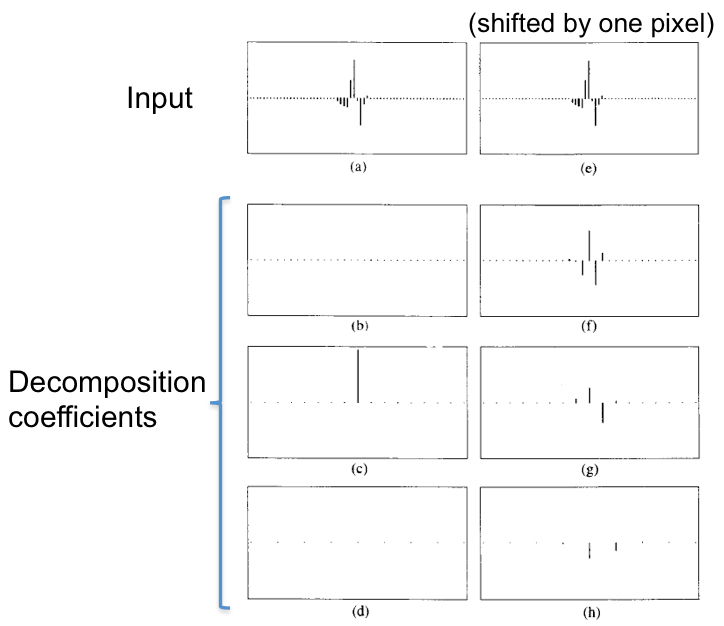
\includegraphics[width=0.6\linewidth]{figures/pyramids/splat.jpg}
%}
%\caption{showing translation variance of an aliased subband representation}
%\label{fig:splat}
%\end{figure}
%
%
%
%
%
\section{Steerable Pyramid}

The Laplacian pyramid provides a richer representation than the Gaussian pyramid. But we would like to have an even more expressive image representation.  The {\bf steerable pyramid} \cite{Simoncelli95} adds information about image orientation. Therefore, the steerable representation is a {\bf multiscale oriented representation} that is translation-invariant. 
\index{Multiscale oriented representation}
It is non-aliased and self-invertible. Ideally, we'd like to have an image transformation that was
shiftable, that is, where we could perform interpolations in position, scale,
and orientation using linear combinations of a set of basis
coefficients.  %The steerable pyramid goes part way there.


We analyze in orientation using a steerable filter bank, shown in \fig{\ref{fig:steerable_pyr_sp3Filters}}.  We form a
decomposition in scale by introducing a low-pass filter (designed to
work with the selected bandpass filters), and recursively breaking the
low-pass filtered component into angular and low-pass frequency
components.   Pyramid subsampling steps are preceded by sufficient
low-pass filtering to remove aliasing.


\begin{figure}[h!]
\centerline{
\includegraphics[width=0.80\linewidth]{figures/pyramids/steerable_pyr_sp3Filters.eps}
}
\caption{Oriented filters and the low-pass kernel used in the steerable pyramid.}
\label{fig:steerable_pyr_sp3Filters}
\end{figure}

\marginnote{One {\bf block} of the steerable pyramid computation.
\\[6pt]
\centerline{
\tikzset{
  block/.style    = {draw, thin, rectangle, minimum height = 1.5em,  minimum width = 1.5em},
  sum/.style      = {draw, circle, minimum size=.4cm}, % Adder
  input/.style    = {coordinate}, % Input
  output/.style   = {coordinate} % Output
}
\begin{tikzpicture}[auto, thin, node distance=.8cm, >=latex]%triangle 45]
%% Drawing the blocks of first level:
\draw
	node [] (x0) {$\mathbf{g}_k$}
	node [input,right of=x0, node distance=0.3cm] (x0p) {}
	node [block, right of=x0p] (b0) {$\mathbf{B}_0$}
         node [block, below of=b0] (b1) {$\mathbf{B}_1$}
         node [block, below of=b1] (bk) {$\mathbf{B}_n$}
         node [block, below of=bk] (L1) {$\mathbf{L}$}
         node [block, right of=L1] (D2) {$\mathbf{D}$}
         node [right of=b0, node distance=1.0cm] (b0out) {$\mathbf{b}_{k,0}$}
         node [right of=b1, node distance=1.0cm] (b1out) {$\mathbf{b}_{k,1}$}
         node [right of=bk, node distance=1.0cm] (bkout) {$\mathbf{b}_{k,n}$}
         node [right of=D2, node distance=1.0cm] (out) {$\mathbf{g}_{k+1}$};
       % Joining blocks. 
	\draw[-](x0) -- node {} (x0p);
	\draw[->](x0p) -- node {} (b0);
	\draw[->](x0p) |- node {} (b1);
	\draw[->](x0p) |- node {} (bk);
	\draw[->](x0p) |- node {} (L1);
	\draw[->](L1) -- node {} (D2);
	\draw[->](b0) -- node {} (b0out);
	\draw[->](b1) -- node {} (b1out);
	\draw[->](bk) -- node {} (bkout);
	\draw[->](D2) -- node {} (out);
\end{tikzpicture}
}
}[-.3in]

To ensure that the image can be reconstructed from the steerable
filter transform coefficients, the filters must be designed so that
their sums of squared magnitudes {\em tile} in the frequency domain.  We
reconstruct by applying each filter a second time to the steerable
filter representation, and we want the final system frequency response
to be flat, for perfect reconstruction.



The following block diagram (\fig{\ref{fig:steerable_pyr_architecture}}) shows the steps to build a two-level steerable pyramid and the reconstruction of the input. The architecture has two parts: (1) the analysis network (or encoder) that transforms the input image $x$ into a representation composed of $r=\left[ b_{0,0},...,b_{0,n}, b_{1,0},...b_{1,n},...,b_{k-1,0},...b_{k-1,n} \right]$ and the low pass residual $g_{k-1}$; and (2) the synthesis network (or decoder) that reconstructs the input from the representation $r$.  

% Definition of blocks:
\begin{figure}[h!]
\centerline{
\tikzset{
  block/.style    = {draw, thin, rectangle, minimum height = 1.5em,  minimum width = 1.5em},
  sum/.style      = {draw, circle, minimum size=.4cm}, % Adder
  input/.style    = {coordinate}, % Input
  output/.style   = {coordinate} % Output
  %x/.style   = {coordinate} % Output
}
%%. DRAWING THE STEERABLE PYRAMID
\begin{tikzpicture}[auto, thin, node distance=.9cm, >=latex]%triangle 45]
% Drawing the blocks of first level:
\draw
	node [] (x0) {$\boldimg$}
	node [input,right of=x0, node distance=0.5cm] (x0p) {}
	node [block, right of=x0p] (b0) {$\mathbf{B}_0$}
         node [block, below of=b0] (b1) {$\mathbf{B}_1$}
         node [block, below of=b1] (bk) {$\mathbf{B}_n$}
         node [block, below of=bk] (L1) {$\mathbf{L}$}
         node [block, right of=L1] (D2) {$\mathbf{D}$};
       % Joining blocks. 
	\draw[-](x0) -- node {} (x0p);
	\draw[->](x0p) -- node {} (b0);
	\draw[->](x0p) |- node {} (b1);
	\draw[->](x0p) |- node {} (bk);
	\draw[->](x0p) |- node {} (L1);
	\draw[->](L1) -- node {} (D2);

% Drawing the blocks of second level:
\draw
	%node [input, right of=D2] (x1) {}
	node [input, right of=D2, node distance=0.5cm] (x1p) {}
	node [block, right of=x1p] (b10) {$\mathbf{B}_0$}
         node [block, below of=b10] (b11) {$\mathbf{B}_1$}
         node [block, below of=b11] (b1k) {$\mathbf{B}_n$}
         node [block, below of=b1k] (L11) {$\mathbf{L}$}
         node [block, right of=L11] (D12) {$\mathbf{D}$};
       % Joining blocks. 
	\draw[-](D2) -- node {} (x1p);
	\draw[->](x1p) -- node {} (b10);
	\draw[->](x1p) |- node {} (b11);
	\draw[->](x1p) |- node {} (b1k);
	\draw[->](x1p) |- node {} (L11);
	\draw[->](L11) -- node {} (D12);

% output nodes
\draw 
	node [right of=D12, node distance=1.25cm] (outl1) {$\mathbf{g}_2$}
	node [above of=outl1] (outb1k) {$\mathbf{b}_{1,n}$}
	node [above of=outb1k] (outb11) {$\mathbf{b}_{1,1}$}
	node [above of=outb11] (outb10) {$\mathbf{b}_{1,0}$}
	node [above of=outb10] (outb0k) {$\mathbf{b}_{0,n}$}
	node [above of=outb0k] (outb01) {$\mathbf{b}_{0,1}$}
	node [above of=outb01] (outb00) {$\mathbf{b}_{0,0}$};

	\draw[->](D12) -- node {} (outl1);
	\draw[->](b1k) -- node {} (outb1k);
	\draw[->](b11) -- node {} (outb11);
	\draw[->](b10) -- node {} (outb10);
	\draw[->](bk) -- node {} (outb0k);
	\draw[->](b1) -- node {} (outb01);
	\draw[->](b0) -- node {} (outb00);
	
% reconstruction blocks
% first level
\draw
         node [block, right of=outl1, node distance=1.25cm] (rU12) {$\mathbf{U}$}
         node [block, right of=rU12] (rL11) {$\mathbf{L}$}
         node [block, above of=rL11] (rb1k) {$\mathbf{B}_n$}
	node [sum, right of=rb1k] (suma1k) {\tiny +}
         node [block, above of=rb1k] (rb11) {$\mathbf{B}_1$}
	node [sum, right of=rb11] (suma11) {\tiny +}
         node [block, above of=rb11] (rb10) {$\mathbf{B}_0$}
	node [sum, right of=rb10] (suma10) {\tiny +};
	 %node [input, right of=D2, node distance=0.5cm] (x1p) {}
	 %node [block, right of=x1p] (b10) {$B_0$}
         %node [block, below of=b10] (b11) {$B_1$}
       % Joining blocks. 
       
	\draw[->](outl1) -- node {} (rU12);
	\draw[->](outb1k) -- node {} (rb1k);
	\draw[->](outb11) -- node {} (rb11);
	\draw[->](outb10) -- node {} (rb10);
	
	\draw[->](rU12) -- node {} (rL11);
	\draw[->](rb1k) -- node {} (suma1k);
	\draw[->](rL11) -| node {} (suma1k);
	\draw[->](rb11) -- node {} (suma11);
	\draw[->](suma1k) -- node {} (suma11);
	\draw[->](rb10) -- node {} (suma10);
	\draw[->](suma11) -- node {} (suma10);
	%\draw[->](x1p) |- node {} (b11);
	%\draw[->](x1p) |- node {} (b1k);
	%\draw[->](x1p) |- node {} (L11);
	%\draw[->](L11) -- node {} (D12);
	
% reconstruction second level
\draw 
         node [block, right of=suma10] (rU02) {$\mathbf{U}$}
         node [block, right of=rU02] (rL01) {$\mathbf{L}$}
         node [block, above of=rL01] (rb0k) {$\mathbf{B}_n$}
	node [sum, right of=rb0k] (suma0k) {\tiny +}
         node [block, above of=rb0k] (rb01) {$\mathbf{B}_1$}
	node [sum, right of=rb01] (suma01) {\tiny +}
         node [block, above of=rb01] (rb00) {$\mathbf{B}_0$}
	node [sum, right of=rb00] (suma00) {\tiny +}
	node [right of=suma00, node distance=1cm] (output) {$\boldimg$};

	\draw[->](suma10) -- node {} (rU02);
	\draw[->](rU02) -- node {} (rL01);
	
	\draw[->](rb0k) -- node {} (suma0k);
	\draw[->](rL01) -| node {} (suma0k);
	\draw[->](rb01) -- node {} (suma01);
	\draw[->](suma0k) -- node {} (suma01);
	\draw[->](rb00) -- node {} (suma00);
	\draw[->](suma01) -- node {} (suma00);
	\draw[->](suma00) -- node {} (output);
	
	\draw[->](outl1) -- node {} (rU12);
	\draw[->](outb0k) -- node {} (rb0k);
	\draw[->](outb01) -- node {} (rb01);
	\draw[->](outb00) -- node {} (rb00);
\end{tikzpicture}
}
\caption{Steerable pyramid architecture.}
\label{fig:steerable_pyr_architecture}
\end{figure}

\Fig{\ref{fig:steerable_pyr_clock}} shows an example of an image and its steerable pyramid decomposition using four orientations and three scales.
The steerable pyramid is a self-inverting overcomplete representation (more coefficients than pixels).

\begin{figure}[h!]
\centerline{
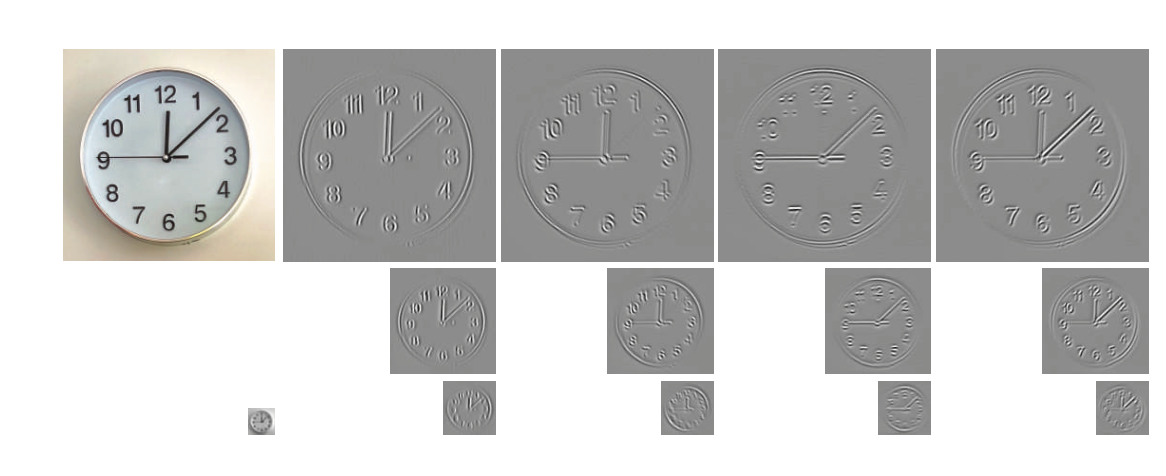
\includegraphics[width=1\linewidth]{figures/pyramids/steerable_pyr_clock.eps}
}
\caption{Steerable pyramid representation (three levels and four orientations). Why is that each orientation subband seems to indicate a different time?}
\label{fig:steerable_pyr_clock}
\end{figure}


%\begin{figure}[h!]
%\centerline{
%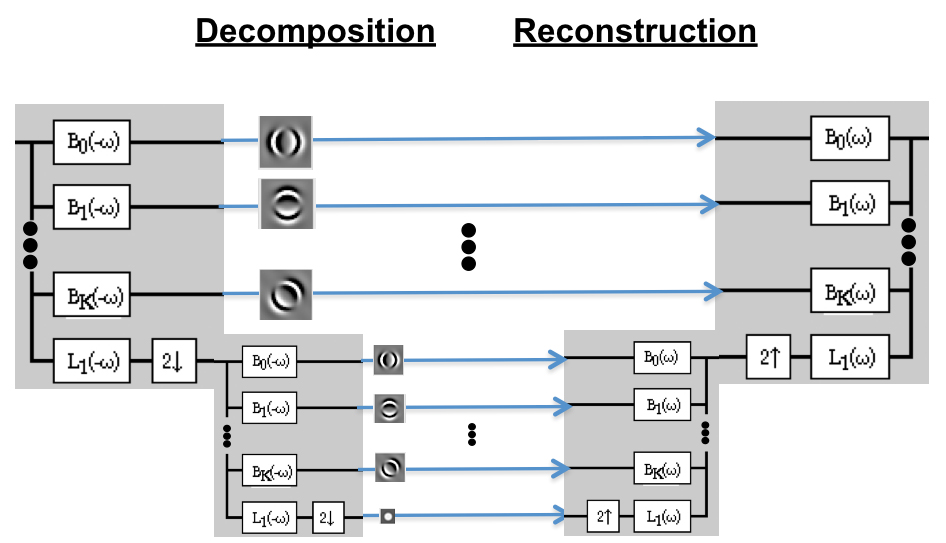
\includegraphics[width=0.7\linewidth]{figures/pyramids/blocksteerpyr.jpg}
%}
%\caption{Steerable pyramid block diagram.}
%\label{fig:blocksteerpyr}
%\end{figure}
%
%


% From Eero toolbox:
%%The steerable pyramid is a multi-scale representation that is
%% translation-invariant, but that also includes representation of
%% orientation.  Furthermore, the representation of orientation is
%% designed to be rotation-invariant. The basis/projection functions
%% are oriented (steerable) filters, localized in space and frequency.
%% It is overcomplete to avoid aliasing.  And it is "self-inverting"
%% (like the QMF/Wavelet transform): the projection functions and 
%% basis functions are identical.  The mathematical phrase for a 
%% transform obeying this property is "tight frame".


%
%
%
%\begin{figure}
%\centerline{
%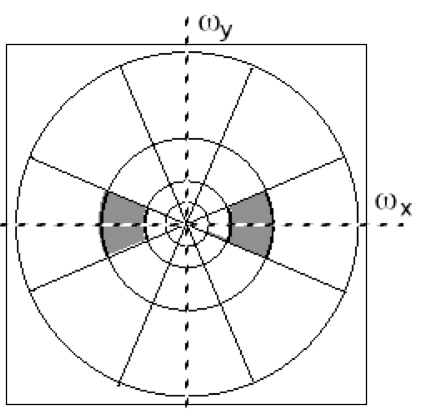
\includegraphics[width=0.4\linewidth]{figures/pyramids/steerpyrfreq.jpg}
%}
%\caption{Steerable pyramid frequency diagram}
%\label{fig:steerpyrfreq}
%\end{figure}
%
%
%There's a mis-match between rotation invariance and the rectangular
%pixel sampling lattice.  The frequency domain is square, but
%a rotationally invariant image representation will have frequency
%subbands arranged as concentric circles, shown in Fig.~\ref{fig:steerpyrfreq}.
%As with the other pyramid image representations, we have a residual,
%unoriented low-pass band, but the steerable pyramid also has a
%high-pass residual subband, as well.
%
%
%\begin{figure}
%\centerline{
%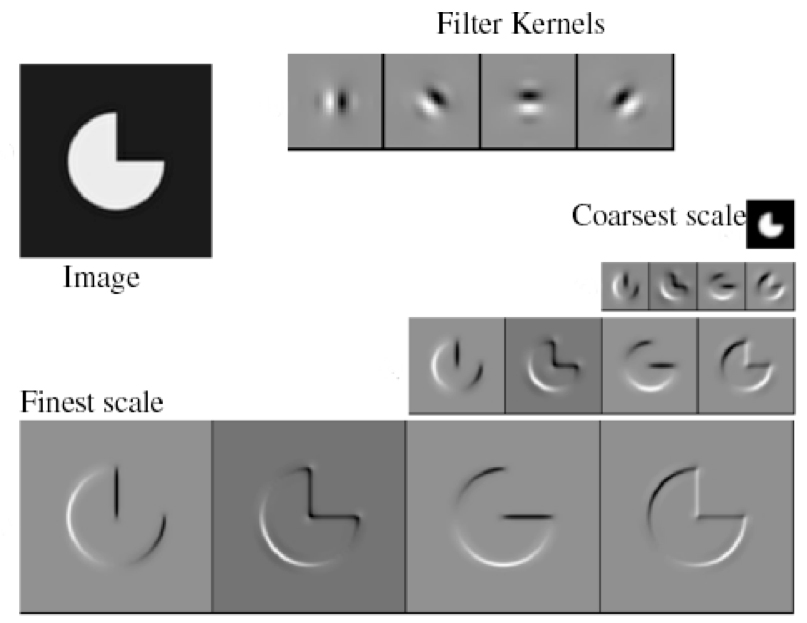
\includegraphics[width=0.7\linewidth]{figures/pyramids/steerpyr.jpg}
%}
%\caption{Steerable pyramid representation.}
%\label{fig:steerpyr}
%\end{figure}
%
%Overall, the steerable pyramid representation is quite overcomplete.
%You can see that in the visualization in Fig.~\ref{fig:steerpyr} of an image and its transform.
%If there are N steerable filters in the representation, then we have N
%images the size of the original at the highest frequency
%representation (plus 1 for the high-pass residual image), and extra
%coefficients are needed to represent the steerable subbands at the
%coarser levels of the pyramid, plus the final low-pass residual image.
%
%So we may not want to use such a representation for image compression
%applications (although the over-complete Laplacian pyramid has been
%used for compression).  But it is useful for various image and texture
%analysis applications, since the subbands represent what they are
%advertised to represent--the signal components in a particular
%frequency band. 
%
%

\section{A Pictorial Summary}

\Fig{\ref{fig:pictorialsummary_pyr}} shows a pictorial summary of the different pyramid representations we've discussed in this chapter.  The figure shows the projection matrices $\mathbf{P}$ for each transformation, both in the 1D case and 2D case. Each projection matrix formed by stacking the projection matrices of each pyramid level.


Figures \ref{fig:pictorialsummary_pyr}(a-c) start with a 1D input signal of length 16. For instance, for a three-level Gaussian pyramid, \fig{\ref{fig:pictorialsummary_pyr}}{b} shows the following projection matrix: 
\begin{equation}
    \mathbf{P} =  
    \begin{bmatrix}
    \mathbf{I} \\
    \mathbf{G}_0 \\
    \mathbf{G}_1 \\
    \end{bmatrix}
\end{equation}
The first block is the identity matrix as the first level is the input image itself. 

For a two-level Laplacian pyramid with a Gaussian residual, the projection matrix $\mathbf{P}$ is (\fig{\ref{fig:pictorialsummary_pyr}}[b]): 
\begin{equation}
    \mathbf{P} =  
    \begin{bmatrix}
    \mathbf{L}_0 \\
    \mathbf{L}_1 \\
    \mathbf{G}_1 \\
    \end{bmatrix}
\end{equation}

The Fourier transform gives a complex-valued output (represented in color) and is global, that is, each output coefficient depends, in general, on every input pixel. The Gaussian pyramid is seen to be banded, showing that it is a localized transform where the output values only depend on pixels in a neighborhood.  It is an overcomplete representation, shown by the transform matrix being taller than it is wide. The Laplacian pyramid is a band-passed image representation, except for the low-pass residual layer, shown in the bottom rows. For this matrix, zero is plotted as gray.  

Figures~\ref{fig:pictorialsummary_pyr}(d-h) show the projection matrices when the input is a 2D image of size $16\times16$ pixels. First, the image is represented as a column vector of length $256=16\times16$ values. \Fig{\ref{fig:pictorialsummary_pyr}}{d} shows the projection matrix of the 2D Fourier transform, a square matrix of size $256\times256$, composed of small blocks of size $16\times16$ that look like 1D Fourier transforms.  Figures~\ref{fig:pictorialsummary_pyr}(e and f) show the Gaussian and Laplacian pyramids, respectively. 

Figures~\ref{fig:pictorialsummary_pyr}(g-h) show the steerable pyramid representation, depending on the number of orientations (\fig{\ref{fig:pictorialsummary_pyr}}[g] is a pyramid with two orientations and \fig{\ref{fig:pictorialsummary_pyr}}[h] has four orientations per scale). The steerable pyramid representation can be very overcomplete (the matrix is much taller than wide). 


The steerable pyramid is an overcomplete, multiorientation representation. We only show the stererable pyramid for 2D images as in 1D, image orientation isn't defined.  The multiple orientations, and non-aliased subbands cause the representation to be very overcomplete, much taller than it is wide. The last block of the steerable pyramid projection matrices computes the low-pass residual.

%All the transforms, except for the Fourier transform, are convolutional, revealed by the diagonal banding in the matrices. 


%
%
%


\begin{figure}[t]
\includegraphics[width=1\linewidth]{figures/pyramids/visualizations_pyr2.pdf}
\caption{Visual comparison of linear transform image representations discussed in this chapter. All the transforms are visualized as a matrix where the number of rows is the size of the input, and the number of columns is the size of the output. All the transforms, except for the Fourier transform, are convolutional, revealed by the diagonal banding in the matrices. 
%Figures (a), (b) and (c) show three transforms for a 1D image of length 16. Each plot shows (a) the Fourier transform, b) the Gaussian pyramid (three levels), and c) the Laplacian pyramid (two levels and the Gaussian residual) respectively. Figures d-h show the projection matrices for transforms of 2D images of size $16 \times 16$. Each plot shows (d) the 2D Fourier transform, (e) the Gaussian pyramid (three levels), and c) the Laplacian pyramid (two levels and the Gaussian residual) respectively, (g) steerable pyramid (2 orientations, 2 levels, and the low pass residual), (h) steerable pyramid with four orientations.
}
\label{fig:pictorialsummary_pyr}
\end{figure}


\section{Concluding Remarks}


To recap briefly, the Fourier transform reveals spatial frequency content of the image wonderfully, but suffers from having no spatial localization. A Gaussian pyramid provides a multiscale representation of the image, useful for applying a fixed-scale algorithm to an image over a range of spatial scales.  But it doesn't break the image into finer components than simply a range of low-pass filtered versions.  The representation is overcomplete that is, there are more pixels in the Gaussian pyramid representation of an image than there are in the image itself.

The Laplacian pyramid reveals what is captured at one spatial scale of a Gaussian pyramid, and not seen at the lower-resolution level above it.  Like the Gaussian pyramid, it is overcomplete. It is useful for various image manipulation tasks, allowing you to treat different spatial frequency bands separately.

The steerable pyramid adds orientation information into the representation, and the representation can be very overcomplete (the matrix is much taller than wide). The steerable pyramid has negligible aliasing artifacts and so can be useful for various image analysis applications.

In image processing applications (i.e., image compression, denoising, etc.) people have used other transforms. For instance, the Haar/wavelet/QMF pyramid \cite{Adelson87b} brings in some limited orientation analysis and different than the other pyramid representations, is complete rather than overcomplete.  This helps it for image compression applications, but hurts it for others because each subband depends on information in other subbands to let it reconstruct the original image without artifacts.  So if you alter one band without altering the corresponding other ones, you can easily introduce artifacts (although artifacts will also appear in overcompleted representations).

\marginnote{Another important framework for multiscale image analysis, not presented in this book,  is {\bf scale space}. 
\index{Scale space}
For an in depth presentation of this topic we direct the reader to \cite{Lindeberg1994}.}


%

%\section{Scale space}






